This chapter is thematically divided into four sections, for each of which a high-level concept or architecture is proposed, that aims to fulfill the requirements stated in \autoref{sec:problem_analysis:goals_requirements}. Various design options are discussed and the proposed system's novelty in comparison to previous approaches is conclusively outlined.

Throughout this chapter, requirements from \autoref{sec:problem_analysis:goals_requirements} are referenced with the prefixes \textit{\textbf{F-}} and \textit{\textbf{NF-}}, respectively.

\section{Environment Modeling \& State Representation}
\label{sec:concept_design:environment_modeling_state_representation}
As stated in \autoref{sec:problem_analysis:goals_requirements}, a major goal of this thesis is to propose a common way to model and represent dynamic traffic scenes with the purpose of being used for cooperative perception. The following sections present challenges, requirements, design decisions and eventually a holistic concept.

In \autoref{subsec:concept_design:object_level_representation_fusion}, the decision for using high-level fusion is motivated and an overview of information to be included in the proposed model is outlined. In \autoref{subsec:concept_design:principle_of_dynamic_world_modeling}, modeling principles to be respected during the design phase are presented. Then, a basic structure / framework is proposed in \autoref{subsec:concept_design:discrete_environment_model_with_occupancy_tiles}, before \autoref{subsec:concept_design:probabilistic_entity_relationship_model_for_cooperative_perception} unveils the complete meta model. 
In \autoref{subsec:concept_design:object_level_representation_fusion}, the decision for using high-level fusion is motivated and an overview of information to be included in the proposed model is outlined. In \autoref{subsec:concept_design:principle_of_dynamic_world_modeling}, modeling principles to be respected during the design phase are presented. Then, a uniform spatial abstraction using Geo tiling is proposed in \autoref{subsec:concept_design:discrete_environment_model_with_occupancy_tiles}, before \autoref{subsec:concept_design:probabilistic_entity_relationship_model_for_cooperative_perception} introduces Probabilistic Entity Relationship models as a way to uniformly incorporate rich semantics and a notion of uncertainty into the model. Eventually, \autoref{subsec:concept_design:the_final_model} unveils the final, comprehensive meta model to be used throughout the course of this work.

\subsection{Object-Level Representation \& Fusion}
\label{subsec:concept_design:object_level_representation_fusion}
As explained \autoref{subsec:background:sensor_fusion}, different abstraction levels of sensor fusion exist to design a cooperative perception system after and both low- and high-level fusion approaches are featured in literature. Chen et al. \cite{Chen2019} favor the exchange of raw data over object-level information and argue that the latter requires a common reference object shared between two vehicles. As will be seen in later sections, this problem does not apply in the context of this work. Instead, high-level fusion is accompanied by benefits that heavily outweigh those of low-level fusion and is the only approach that allows to fulfill this work's requirements. \autoref{tab:comparison_fusion} presents are detailed comparison of these two principles with regard to benefits and drawbacks.

\begin{table}[H]
	\centering
	\begin{tabular}{|p{7.5cm}|p{7.5cm}|}
		\hline
		\textbf{Advantages} & \textbf{Disadvantages} \\ \hline
		Significantly smaller data volumes, latency and network utilization \textbf{(NF-M3)} & Need for a common, shared model \\ \hline
		Significantly lower computational load at observer vehicles \textbf{(NF-M3)} & Potential need for schema versioning \\ \hline
		Independent of sensor type, characteristics and calibration \textbf{(NF-M1, NF-M2)} & \multirow{3}{*}{} \\ \cline{1-1}
		Support for different levels of abstraction (e.g. to include semantic information about pair-wise relations among traffic participants) \textbf{(F-M1, F-M2)} &  \\ \cline{1-1}
		Allows for inference without further processing \textbf{(NF-M2, NF-M3)} &  \\ \hline
	\end{tabular}
	\caption[Comparison High-/Low Level Fusion]{Advantages of High-Level Fusion over Low-Level Fusion for Cooperative Perception. Requirements are referenced, whose fulfillment the respective advantage enables for.}
	\label{tab:comparison_fusion}
\end{table}

When using a high-level object model, the most essential part to be defined is the information the model is supposed to include. \cite{Petrich2018} states that \textit{"'a traffic scene is described by the entities, their attributes and the relations among the entities"'}. Following this definition and in order for the model to be as expressive (\textbf{F-M1}) as possible, the model is meant to include:

\begin{itemize}
	\item State and topology of the immediate static environment and road
	\item State, static- and dynamic properties for both the ego vehicle itself and all surrounding traffic participants
	 network
	\item Relations among any kinds of entities within the ego vehicle's immediate surrounding (e.g. vehicle-vehicle-, or vehicle-traffic-light relations)
\end{itemize}

Especially the inclusion of semantic, relational information – originally proposed by \cite{Kohlhaas2014} – in novel compared to all previously presented CP systems. \autoref{fig:relations} depicts a minimal example of such relations. 

\begin{figure}
	\centering
	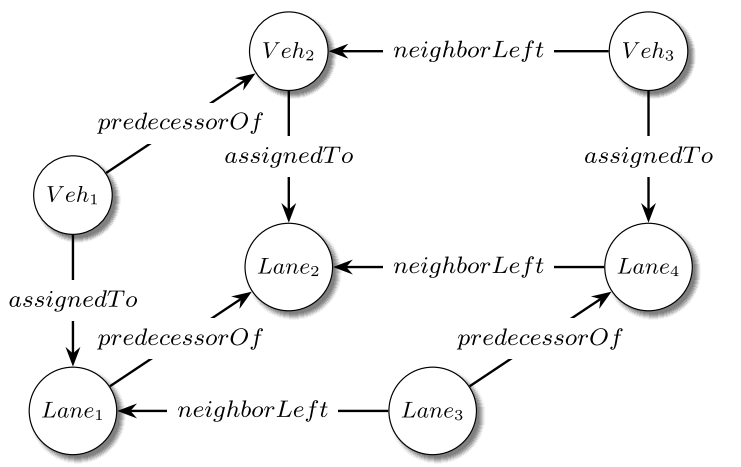
\includegraphics[width=0.5\linewidth]{98_images/relations}
	\caption[Semantic Relations between Traffic Participants]{Illustration of a Graph of Semantic Relations between Traffic Participants \cite{Petrich2018}}
	\label{fig:relations}
\end{figure}

\subsection{Principles of Dynamic World Modeling}
\label{subsec:concept_design:principle_of_dynamic_world_modeling}

\begin{samepage}
	Modeling road traffic requires the ability to capture and integrate perceptual information of highly dynamic environments properly – a problem for which \cite{Crowley1993} states five essential principles. In the following, the original term \textit{"'primitive"'} is substituted by \textit{"'entity"'}. 
	
	\begin{enumerate}[\ \ P1:]
		\item Entities in the world model should be expressed as a \textbf{set of properties}.
		\item Observation and model should be expressed in a \textbf{common coordinate system}.
		\item Observation and model should be expressed in a \textbf{common vocabulary}.
		\item Properties should include an \textbf{explicit representation of uncertainty}.
		\item Entities should be accompanied by a \textbf{confidence factor}.
	\end{enumerate}
\end{samepage}

This principles are picked up again for the concrete model specification presented later.

\cite{Crowley1993} also presents a "'General Framework for Dynamic World Modeling"', depicted in \autoref{fig:dynamic_world_modeling} (left). It illustrates the high-level process to transform heterogeneous types of observations into a unified model using a common vocabulary. The process includes a \textit{Match-Update-Predict} cycle, the purpose of which is to enhance observations with evidence derived from previous observations and a prediction model. Although especially the \textit{Match} step is quite essential for a real-world system, it is neglected in this thesis for the sake of focusing on the higher-level system architecture. Instead, a simplified process (right) is applied.

Throughout the course of following sections, the above principles are referenced using the respective \textit{\textbf{P}} prefixes.

\begin{figure}
	\centering
	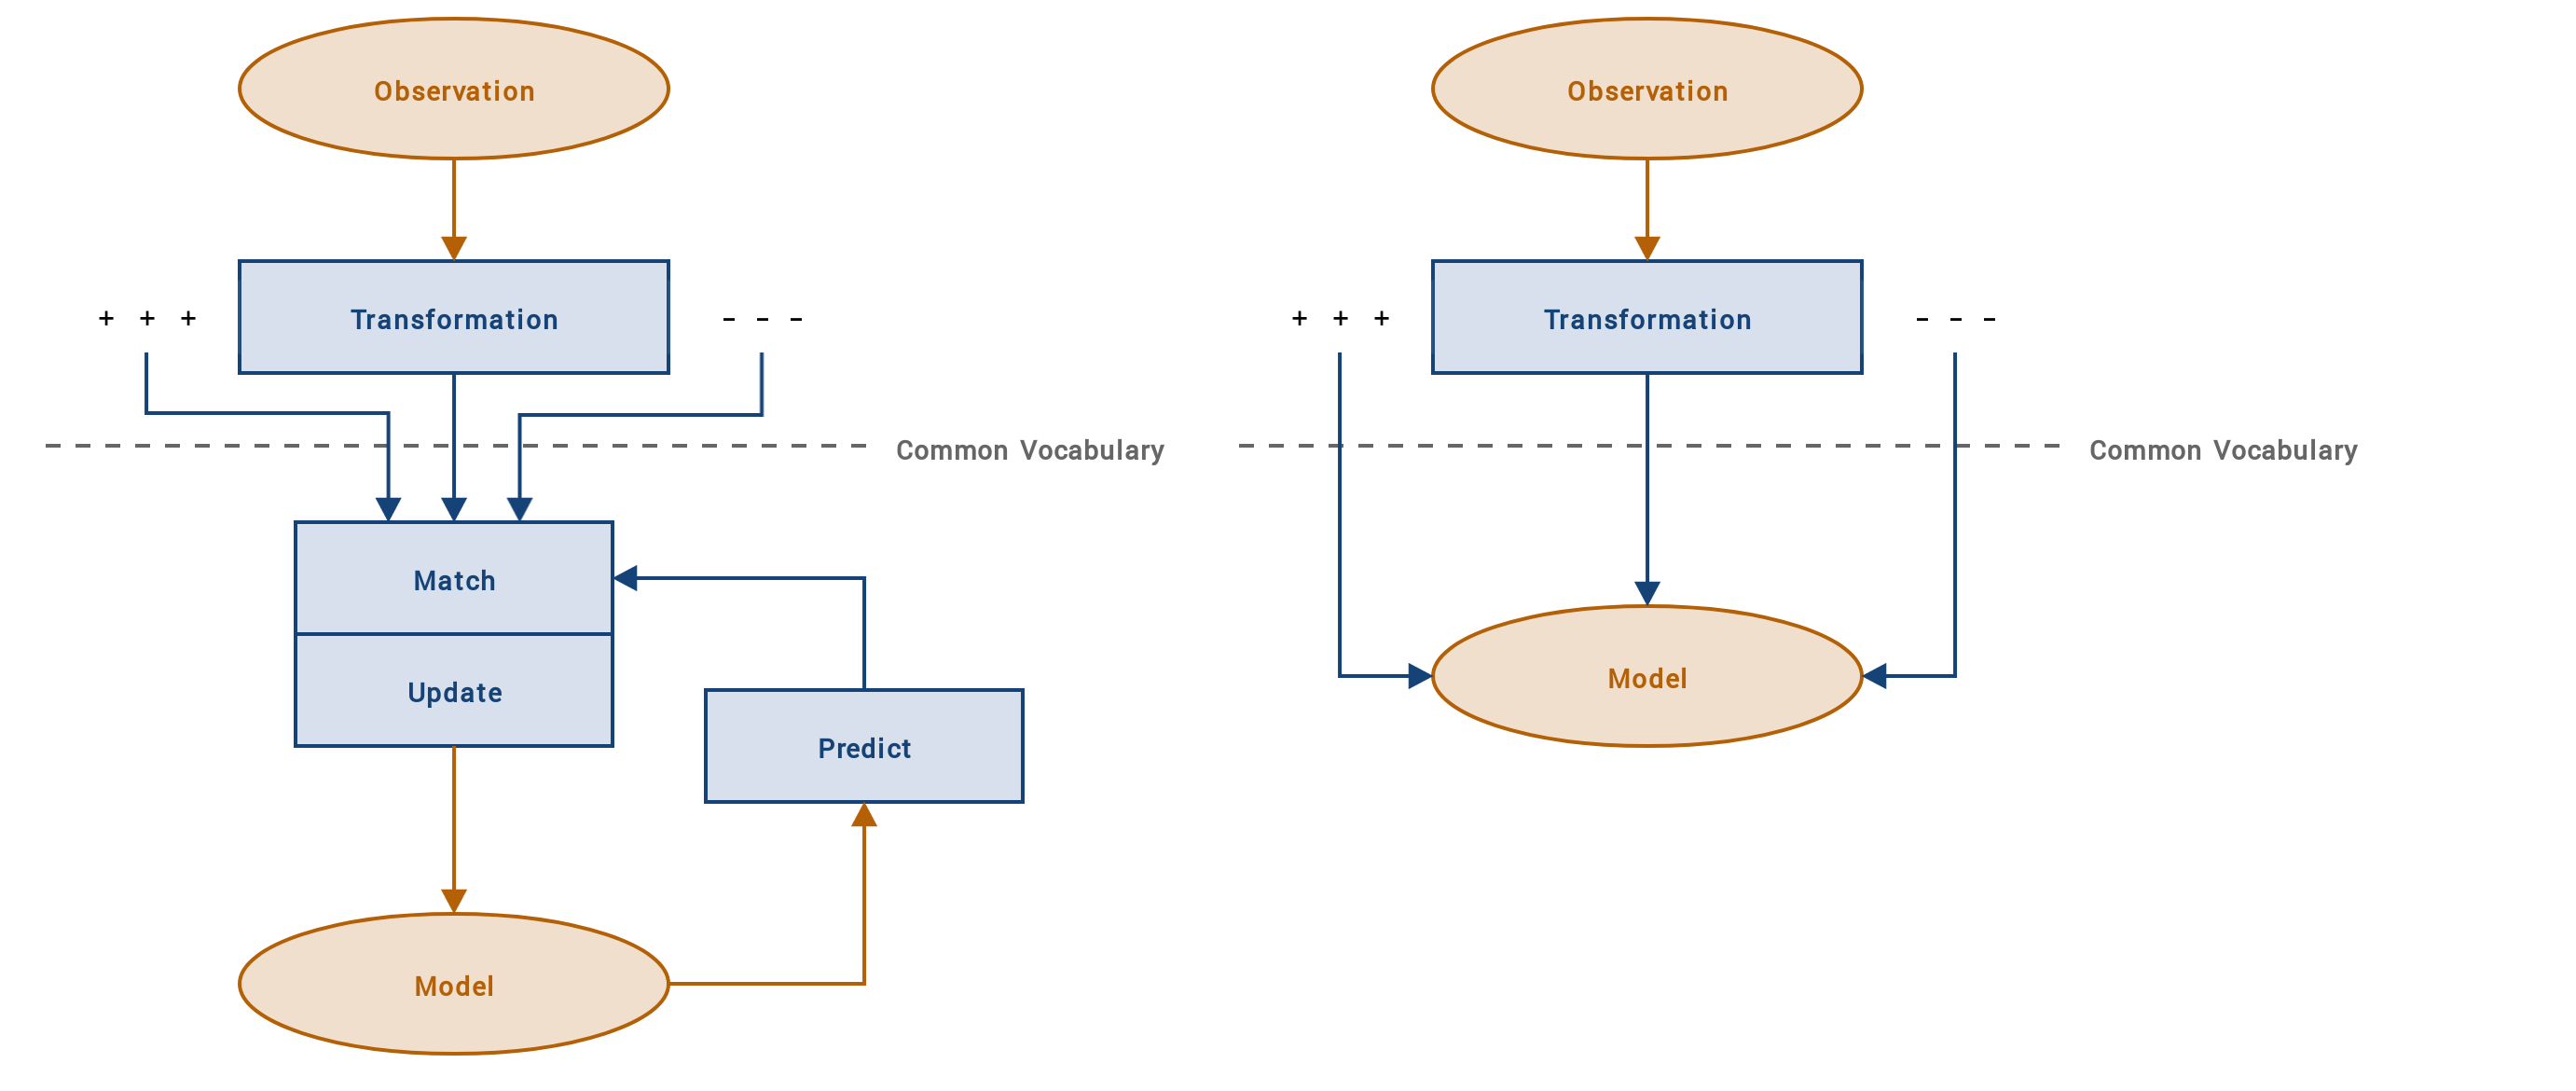
\includegraphics[width=1.0\linewidth]{98_images/dynamic_world_modeling}
	\caption[General Framework for Dynamic World Modeling]{General Framework for Dynamic World Modeling \cite{Crowley1993} (left: original, right: simplified version used in this thesis)}
	\label{fig:dynamic_world_modeling}
\end{figure}

\subsection{Discrete Environment Model with Occupancy Tiles}
\label{subsec:concept_design:discrete_environment_model_with_occupancy_tiles}

When attempting to model one's neighboring traffic environment, a mental distinction can be made into modeling the road network – including lane topology, traffic lights, sidewalks, etc. – and modeling static and dynamic obstacles, like other vehicles, pedestrians or trees. Both aspects are needed for a complete representation, as it is neither sufficient to only know the course of the road nor to only be aware of obstacles. Moreover, it is not sufficient to solely know an obstacle's position, but instead one is usually interested in more advanced properties, too. This work aims to combine all of these aspects in a shared model to enable them for being perceived cooperatively. Accordingly, the idea of \cite{Rauch2011} to share an object list is combined with the concept of \cite{liu2013motion} to share a discretized driveability map, also known as \textit{occupancy grid}. 
\par
\bigskip

The very base of our proposed model is made up of cells of an \textbf{occupancy grid} with fixed dimensions. Such can be constructed by any observer (vehicle, RSU, etc.) and derived from any kind of perceptual sensor data. This simplification facilitates universality \textbf{(NF-M1)}. However, these basic information can be enriched with more complex features easily to support expressiveness \textbf{(F-M1)}. This is achieved through the use of a graph-based meta model, as explained in \autoref{subsec:concept_design:probabilistic_entity_relationship_model_for_cooperative_perception}.

To work towards the perspicuity \textbf{(NF-M2)} requirement and to follow the principle of using a common coordinate system (\textbf{P2}), every cell is identified by a \textbf{QuadKey}. As a consequence, referring to a cell's position is independent from local, per-vehicle coordinates systems and from the GNSS / GPS coordinate frames alike. This prevents network participants from a multitude of expensive transformation operations.

Following this concept, the entire world map is recursively split into QuadTiles (see \autoref{sec:background:geo_tiling}) of a certain precision level (e.g. level 24, corresponding to square tiles of \textasciitilde\SI{2.39}{\square\meter}). The precision level should be chosen in a way that it is fine-grained enough to distinguish between single pedestrians or even road signs. However, at the same time, it must not be too exact to save bandwidth and computation load.

Each cell of the occupancy grid – one of which is observed locally by every connected participant – then corresponds to a certain QuadTile. Besides its occupancy state, every tile can be augmented with information like the corresponding occupant actor, its relation to the overall road topology, etc. 

\autoref{fig:tiling1} illustrates the proposed \textit{occupancy tile} concept. The blue grid is within the observation range of the turquoise vehicle and inherently part of larger tiles. Each cell's (= each tile's) state is determined through local sensor fusion involving different types of in-vehicle sensors and can be extended by additional information. Eventually, that grid, entailing all relevant information, is shared with other CP participants.

\begin{figure}[h]
	\centering
	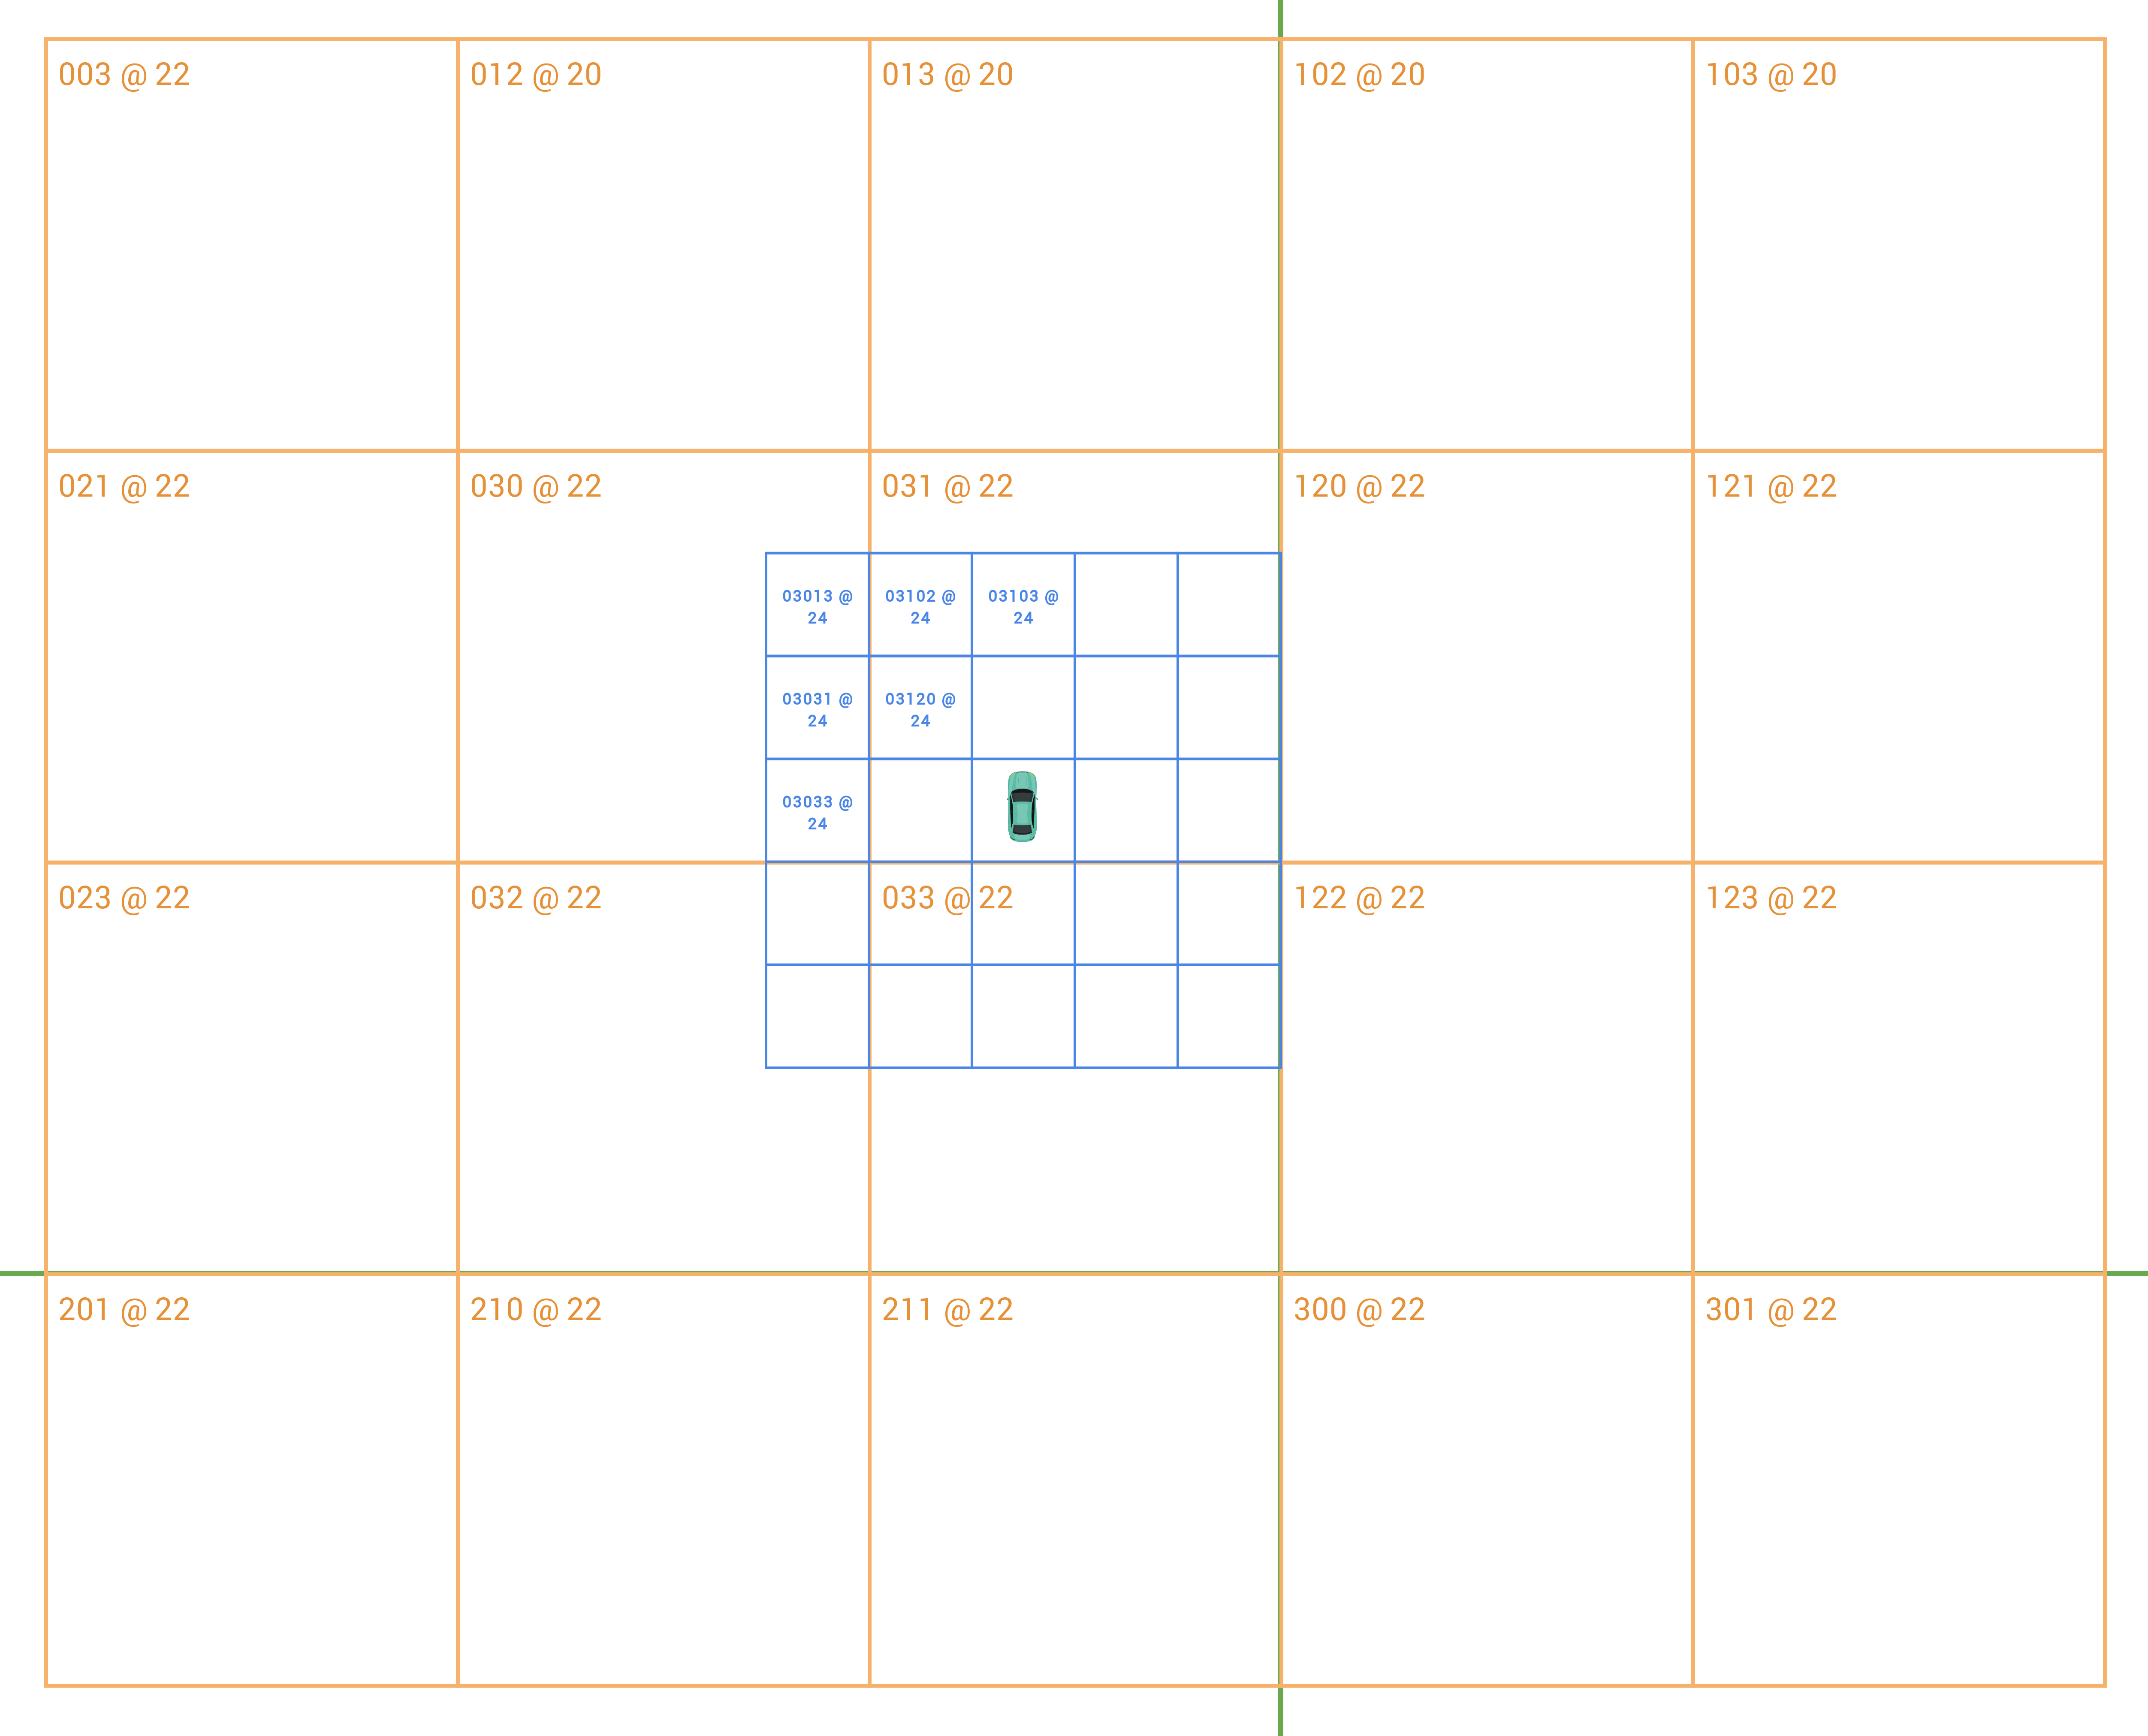
\includegraphics[width=1.0\linewidth]{98_images/geo_subscription_schema_1}
	\caption{Illustration of an Occupancy Grid using QuadTiles}
	\label{fig:tiling1}
\end{figure}


\subsection{Probabilistic Entity Relationship Model for Cooperative Perception}
\label{subsec:concept_design:probabilistic_entity_relationship_model_for_cooperative_perception}

In the simplest case, each observed cell of the previously introduced occupancy holds only information on whether it is occupied or not. However, this  piece of data is usually insufficient to extensively describe a road scene. In addition, object-level static- (e.g. type, color and extent) and dynamic (e.g. velocity- and acceleration) information are desirable, e.g. about the occupying obstacle. This is in line with the requirements to support expressiveness \textbf{(F-M1)} openness \textbf{(F-M2)} and can be taken even one step further. To do so, \cite{Kohlhaas2014, Petrich2018} motivate the idea to also include high-level semantic information about the relationships between different entities in a scene to reduce complexity and help generalization. 

Up to this point, it is coarsely specified \textit{what} to incorporate into the model: static and dynamic properties of each entity within the scene on different levels of abstraction – including semantics – using occupancy tiles as base- or root entities. The second step is to specify \textit{how} to represent these. Previous requirements imply a structure in which \textbf{entities} have \textbf{attributes} (or properties, see principle \textbf{P1}) and \textbf{relations} of various types among different entities can exist. Additionally, in order to appropriately meet the inherently uncertain nature of a partially observable environment using imperfect sensory and to comply with principles \textbf{P4} and \textbf{P5}, some notion of \textbf{confidence} needs to be incorporated into the model. A way is needed to probabilistically model an observer's belief in the truthfulness of a particular property value or the existence of a certain relation between entities. 

These needs lead to the introduction of \textbf{Probabilistic Entity Relationship Models} (PER models). Such are already used by \cite{Petrich2018} for traffic scene representation and can be seen as an extension to regular Entity Relationship Models (ER models). Correspondingly, they incorporate the notion of entities with attributes and inherently define entity-entity relations. Both entity-attribute combinations and entity-entity relations can be represented as $\langle subject, predicate, object \rangle$ triples:

\begin{gather}
	r \in \{ \langle \mathcal{E} \times \mathcal{A} \cup \mathcal{R} \times \mathcal{E} \cup \mathcal{L} \rangle \}
\end{gather}
\label{eq:triples}

$\mathcal{E}$ is the set of all entities, $\mathcal{A}$ is the set of all attributes, $\mathcal{R}$ is the set of all entity-entity relations and $\mathcal{L}$ denotes a literal, i.e. a number, boolean value or string.

With PER models, every triple is extended with an additional confidence parameter and thus becomes a \textbf{quadruple} $r$ of $\langle subject, predicate, object, \textit{conf} \rangle$: 

\begin{gather}
	r \in \{ \langle \mathcal{E} \times \mathcal{A} \cup \mathcal{R} \times \mathcal{E} \cup \mathcal{L} \times \Gamma \rangle \} \\
	\text{with} \  \Gamma := \{ \gamma \in [0, 1] \subset \mathbb{R}^+ \} \\
\end{gather}
\label{eq:quadruples}

\cite{Petrich2018} distinguishes between \textit{attribute-} and \textit{structure uncertainty}, where the first describes sensor noise and the latter reflects uncertainty in the relational data. This is analogous to principles \textbf{P4} and \textbf{P5}, which suggest to model uncertainty for properties on the one hand and a confidence factor for entities on the other. However, this distinction is not considered useful in the context of this work and thus both probabilities are subsumed under a single notion of confidence.

An exemplary excerpt from an instantiated PER model, that was constructed based on observations of some ego vehicle, might look like this:

\begin{gather*}
	\langle \textit{obstacle\_25}, \textit{isOfType}, \textit{"'small\_car"'}, 0.921 \rangle \\
	\langle \textit{obstacle\_25}, \textit{hasVelocity}, (0.65, 0.42, 0), 0.448 \rangle \\
	\langle \textit{obstacle\_25}, \textit{isStoppedAt}, \textit{traffic\_light\_190}, 0.995 \rangle
\end{gather*}

In the example, $\textit{obstacle\_25}$ and $\textit{traffic\_light\_190}$ are entities, which were perceived, identified and tracked by an intelligent vehicle's sensory. $\textit{isOfType}$ and $\textit{hasVelocity}$ are attribute relations with attributes literals (string and three-dimensional numeric vector) and $\textit{isStoppedAt}$ stands for an entity-entity relation.

Such relations can be separated into seven classes: \textit{inclusion}, \textit{possession}, \textit{attachment}, \textit{attribution}, \textit{antonym}, \textit{synonym} and \textit{case} \cite{Storey1993}. Three of those are considered relevant for modeling in AD contexts \cite{Petrich2018}.

\begin{itemize}
	\item \textbf{Inclusion:} Indicates structural- or spatial inclusion or class inheritance. \\ Example: $\langle  cross\_walk\_12, isPartOf, lane\_30, \gamma \rangle$
	\item \textbf{Attachment:} Indicates structural- or spatial connection or intersection. \\ Example: $\langle car\_1250, drivesOn, lane\_30, \gamma \rangle$
	\item \textbf{Case:} Indicates interaction or dependence between entities or association of attributes and entities. \\ Examples: $\{ \langle car\_1250, isStoppedAt, traffic\_light\_190, \gamma \rangle, \langle bicycle\_370, hasColor, \\ "'yellow"', \gamma \rangle \}$
\end{itemize}

While relations from any of these classes are represented equally in an PER model, the distinction can help to achieve a clean meta model or database design.
\par
\bigskip

Using quadruples, a PER model is representable as a graph and thus can quite easily be searched, transformed and extended by inserting new relations. Also, the PER can – under certain conditions – be efficiently (\textbf{NF-M3}) represented as a tensor \cite{Petrich2018}.

The graphical representation also allows for different types of inference. New facts about the local world could be inferred when used in combination with first-order logic. Also, situations might easily be compared in terms of similarity, which can be used for case-based reasoning. \cite{Nickel2016} presents a multitude of further techniques to perform relational machine-learning on knowledge graphs, which might prove promising in AD contexts as well. 

\subsection{The Final Model}
\label{subsec:concept_design:the_final_model}
The complete model proposed as part of this thesis is presented in \autoref{fig:final_model}. It aims to be sufficiently comprehensive and includes all aspects needed for an in-depth evaluation of cooperative perception. However, the presented version is still not 100 \% complete. Future work in cooperation with expert groups is desirable to further extend it. 

In the illustration, blue boxes denote entities, orange boxes stand for uncertain entity-entity relations and green circles are uncertain attributes (or entity-literal relations). Gray boxes are special in a way that they can not be subject to instantiation, but rather define the meta model's static structure as a class hierarchy. Filled blue boxes are not of a special meaning, except that they usually occur particularly frequently.

In an instantiation of this model, quadruples include entities (blue) as subject or as subject and object and relations (orange) or attributes (green) as predicate. 

It is worth noting that, in contrast to most prior work in this field, the occupancy state of a cell is modeled \textbf{ternary} instead of binary. An additional bit is used to distinguish between a cell being \textit{free} or \textit{occupied} or just \textit{unknown}. This distinction adds valuable information for the participants of CP network, as an  \textit{unknown} (or \textit{unseen}, \textit{covered}, \textit{beyond-LOS}) state can simply be substituted during the fusion step. In a situation where two vehicles are driving in line (depicted in \autoref{fig:blocked_los_scenario}), the rear car might observe the cells occupied by the leader as occupied. However, there is no chance it can see through the leader car and thus all cells in front of it need to be communicated as being unknown, as opposed to either free or occupied.

\begin{figure}[h]
	\centering
	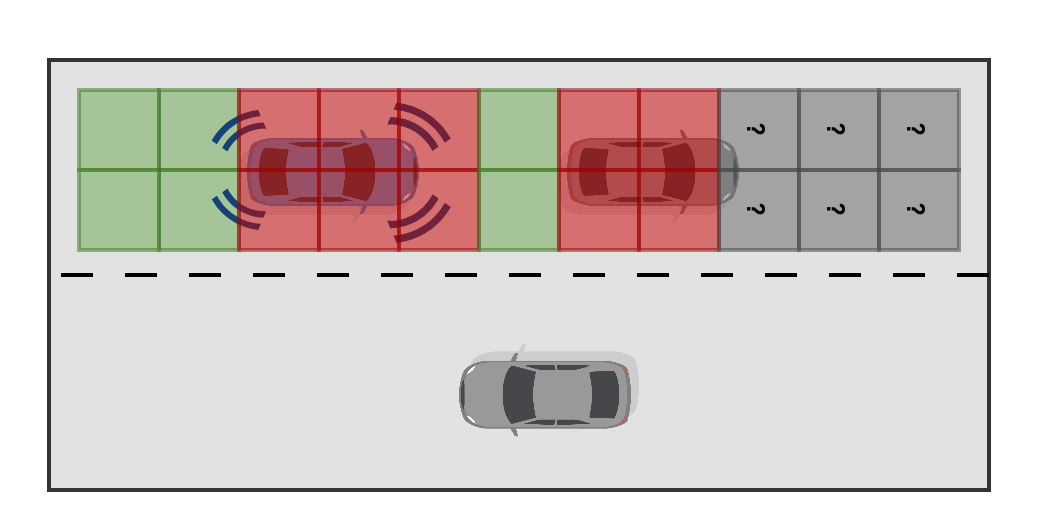
\includegraphics[width=0.7\linewidth]{98_images/unknown_cells_scene}
	\caption{Blocked Line of Sight Scenario}
	\label{fig:blocked_los_scenario}
\end{figure}


In addition, the presented model is rich in a way that ...

\begin{samepage}
	\begin{itemize}
		\item ... it defines a large variety of different entities and relations.
		\item ... it allows to exhaustively specify a cell's occupancy state.
		\item ... features different levels of abstraction (low-level attributes, high-level semantic relations).
		\item ... incorporates class hierarchies as known from object-oriented programming (e.g. $\langle Vehicle, isA, DynamicObstacle \rangle$).
	\end{itemize}
\end{samepage}

A minimal instantiation of this model has to include an \textit{OccupancyGrid} instance with an observer (\textit{observedBy}) \textit{Element} (e.g. a \textit{Vehicle}) and  $1..n$ \textit{GridCells}. How many cells exactly a grid consists of (grid size) can be configured and depends on its observer's sensor range. Each cell has to have at least its \textit{state} and \textit{positionHash} (as a QuadKey) defined. The ternary state can be represented using two bits, its \textit{positionHash} fits into 64 bits when using a QuadKey's integer representation (see \autoref{subsec:background:quadkeys}) and the confidence $\gamma$ would usually be implemented as a 32-bit float. Accordingly, one cell could be modeled using 98 bits in an optimal, minimalist case, what contributes to efficiency (\textbf{NF-M3}).

\begin{sidewaysfigure}
	\centering
	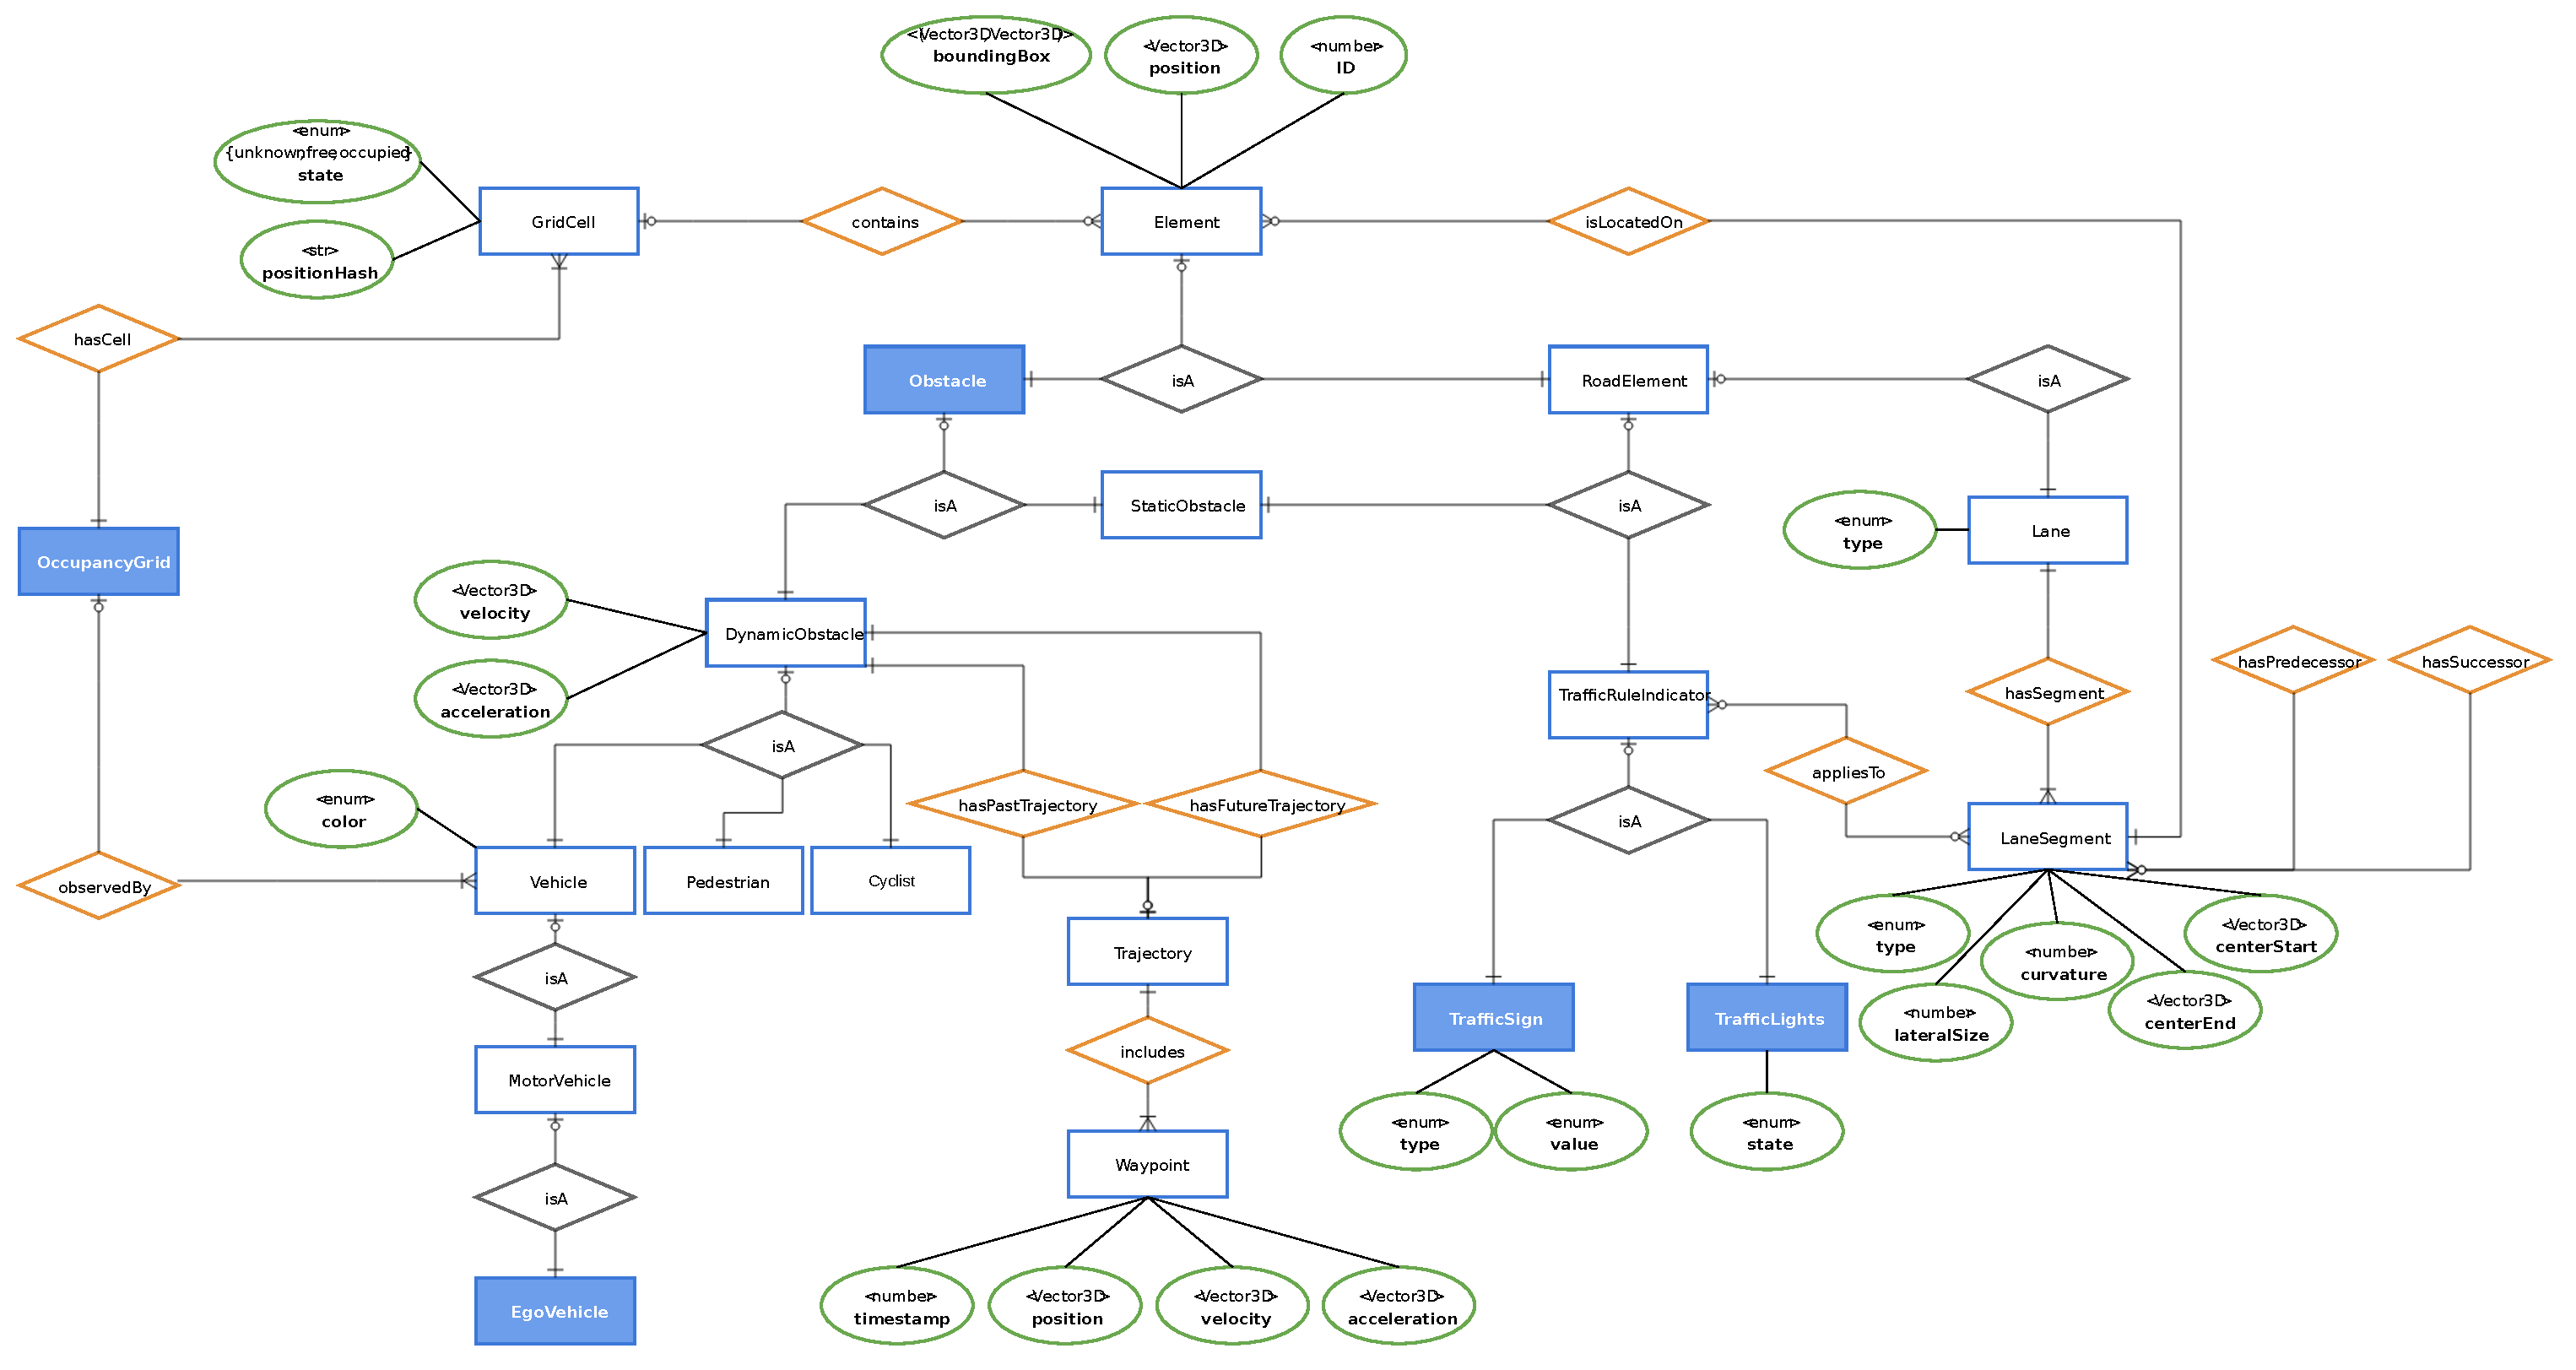
\includegraphics[width=\linewidth]{98_images/scene_representation_er}
	\caption{Comprehensive PER Model for Traffic Scenes}
	\label{fig:final_model}
\end{sidewaysfigure}

\subsection{Summary}
\label{subsec:concept_design:modeling:summary}
In the previous sections a comprehensive, yet not complete, model for dynamic traffic scenes and with a focus on cooperative perception use cases was presented (see \autoref{fig:final_model}). It enable to describe a scene combining low level attributes with high level relational knowledge in a generic way and fulfills the requirements stated in \autoref{sec:problem_analysis:goals_requirements} and follows the modeling principles introduced in \autoref{subsec:concept_design:principle_of_dynamic_world_modeling}.

As a result, it is capable of uniformly and universally modeling road scenarios at a high degree of expressiveness, while embracing a notion of uncertainty or confidence and information on different abstraction levels. Key concepts used include \textbf{geo tiling} based on \textbf{QuadKeys} for spatially referencing cells of an \textbf{occupancy grid} and \textbf{Probabilistic Entity Relationship models} as a structural framework.

\section{Cellular Communication}
\label{sec:concept_design:cellular_communication}
Various downsides of DSRC-based ad-hoc networks for cooperative perception use cases were already discussed in \autoref{sec:problem_analysis:limitations_of_prior_work}. They include issues arising from limited throughput and comparatively short range of IEEE 802.11p and similar technologies. Furthermore, P2P topologies usually imply a large communication overhead and result in high computational load for each participant. To overcome these limitations, an alternative approach is proposed that builds on 5G networks and a client-server topology.

This section briefly presents characteristics, key benefits and implications of 5G technology for V2X communication and motivates the decision for its use in the present CP system.

\subsection{5G Characteristics \& Advantages}
\label{subsec:concept_design:5g_characteristics_advantages}
5G stands for the fifth generation cellular network standard and is the successor of 4G, or LTE. It may be operated on a variety of different spectrums, ranging from low-band (\textasciitilde 600 Mhz) over mid-band (2.4 to 4.2 \si{\giga\hertz}) to millimeter waves in the high-band spectrum ranging from 24 to 72 \si{\giga\hertz}. Which spectrum is used depends mainly on the carrier and has direct influence on communication range and speed. While millimeter wave frequencies will mainly be used in North America, Europe will rely on the low- and mid-range bands.

In networks based on the most widely used mid-band spectrum, average throughput is between 100 and 400 \si{\mega\bit\per\second}, while it can increase up to \SI{2}{\giga\bit\per\second} with millimeter waves \cite{wiki:5g}.

Typical round-trip (RTT) were measured to range from 25-35 \si{\milli\second} and might be improved to 10-20 \si{\milli\second} when employing an \textit{Edge Node} (see \autoref{sec:background:edge_computing}) close to a cell tower \cite{wiki:5g}. Under lab conditions, even less than \SI{1}{\milli\second} latencies were observed.

Like 4G, 5G is based on network cells between which moving mobile clients are handed over. Generally, network cells are smaller with 5G than with 4G, especially in densely populated areas. Depending on which frequency band is used, cell towers may need to be placed every few hundred meters to achieve full coverage.

\cite{5GAutomotiveAssociation2016} presents a detailed, technical discussion of 5G vs DSRC for V2X, while a higher-level comparison with respect to key implications for CP is presented in \autoref{tab:5g_dsrc_comparison}.
\par
\bigskip

ETSI identified three different main usage scenarios for 5G \cite{ETSI5G}, all of which require different key capabilities, as shown in \autoref{fig:5g_capabilities}. The different usage scenarios are:

\begin{itemize}
	\item \textbf{Enhanced Mobile Broadband (eMBB)} to be used for high-definition, low-latency multimedia content and mobile games on end-user devices and smartphones.
	\item \textbf{Massive Machine-type Communications (mMTC)} for the Internet of Things, which is characterized by low-power devices and low data rates.
	\item \textbf{Ultra-reliable and Low Latency Communications (URLLC)} for safety- and mission-critical applications, like autonomous driving. 
\end{itemize}

Cooperative perception requires URLLC and thus especially low latency and high throughput.

\begin{figure}[h]
	\centering
	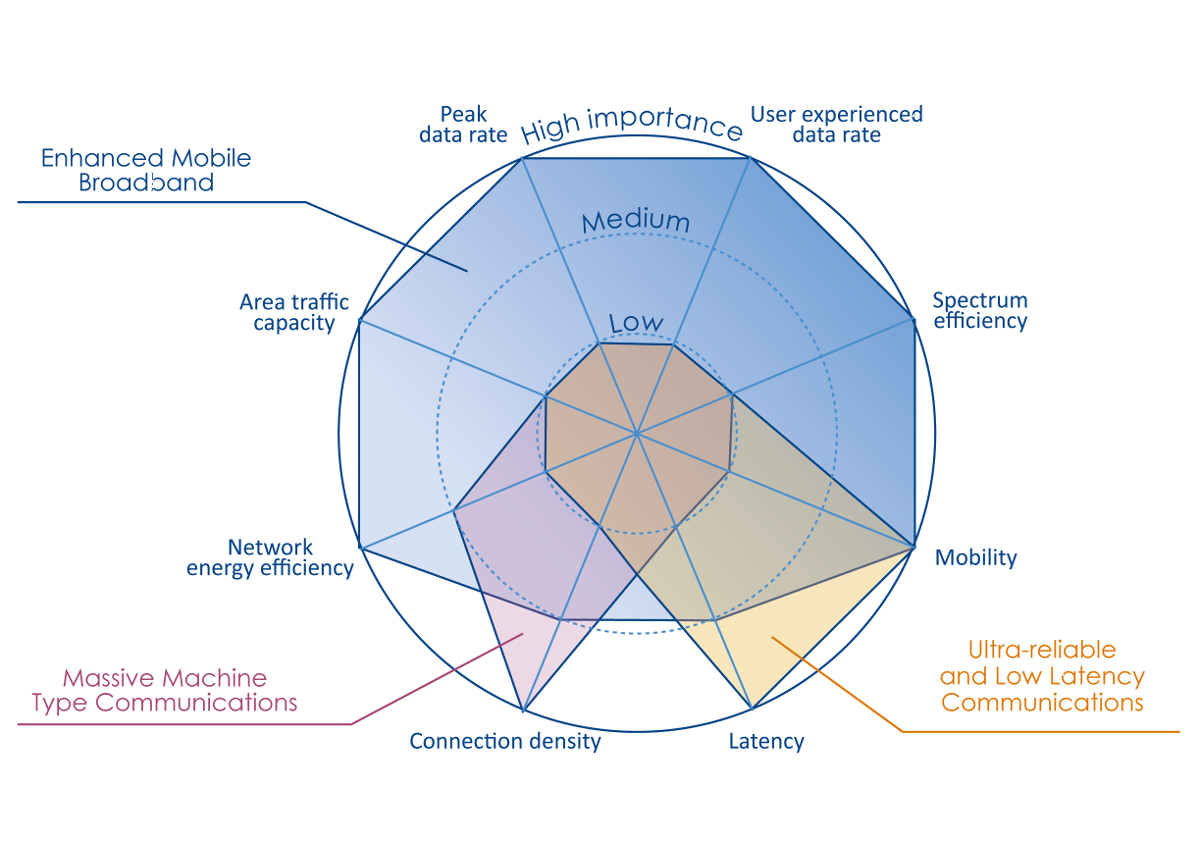
\includegraphics[width=0.75\linewidth]{98_images/5g_spider_chart}
	\caption[Key Capability Requirements for 5G]{Key Capability Requirements for 5G in different Scenarios \cite{ETSI5G}}
	\label{fig:5g_capabilities}
\end{figure}

\subsection{Vehicle-to-Network-to-Everything Communication Topology}
\label{subsec:concept_design:communication_topology}
Most prior work on V2X employs ad-hoc networks (VANETs) between participants, many of which imply a peer-to-peer network topology, i.e. every participant connects to every other participant, following \textit{Metcalfe's Law}. Downsides of such approaches were briefly outlined in \autoref{sec:problem_analysis:limitations_of_prior_work} and mainly refer to scalability and communication overhead.

In order to unburden participant vehicles (or pedestrian smartphones, RSUs, etc.), this work proposes the use of a \textbf{client-server architecture}. Every client connects to a central server instance, that is responsible for its current geographical area, which performs all computation tasks (mainly high-level sensor data fusion) and is responsible for collecting and broadcasting their messages. While the server node has to be very strong in terms of computational capacity, every client now only has to maintain one bi-directional connection and process (e.g. fuse) messages from one sender. \autoref{fig:communication_topology} illustrates both patterns in a scenario of $n = 4$ vehicles. The pattern of V2X now becomes, strictly speaking, V2N2X, as an intermediate network is involved. However, for the sake of simplicity, the term \textit{V2X} will still be used to describe this new pattern. 

Although 5GAA specify multiple transmission modes for 5G \cite{5GAutomotiveAssociation2016} – including \textbf{direct communication} between network clients (V2V in the narrow sense ot the word) – this thesis focuses on V2N-based communication to best counter the previously mentioned drawbacks. 

\begin{figure}[h]
	\centering
	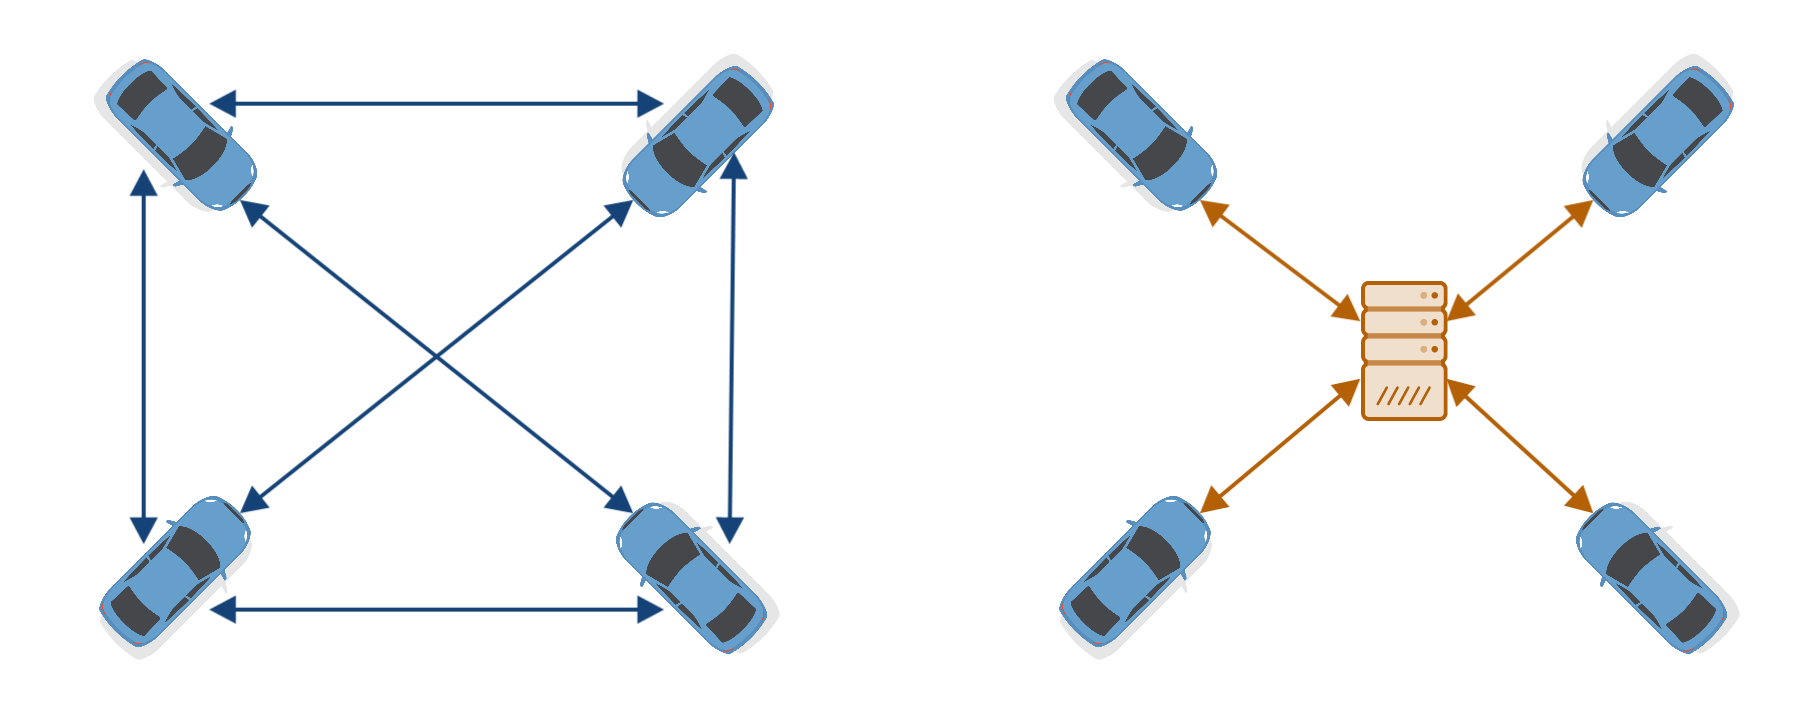
\includegraphics[width=0.9\linewidth]{98_images/topology_comparison}
	\caption{VANET vs. Client-Server Communication Topology}
	\label{fig:communication_topology}
\end{figure}


\subsection{Summary}
\label{subsec:concept_design:5g:summary}
In contrast to most prior work, the CP system developed in the context of this thesis does not rely on DSRC-based VANETs, but on cellular 5G communication with centralized server instances instead. Motivation for this decision was given in previous sections and is additionally summarized in \autoref{tab:5g_dsrc_comparison}.

\begin{table}[H]
	\begin{tabular}{|p{7.6cm}|p{7.6cm}|}
		\hline
		\textbf{VANETs + DSRC}                & \textbf{Client-Server + C-V2X}                                                 \\ \hline
		\rowcolor[HTML]{9AFF99} 
		+ Works anywhere                      & \cellcolor[HTML]{FFCCC9}– Requires network infrastructure and -coverage              \\ \hline
		\rowcolor[HTML]{9AFF99} 
		+ Free of charge                      & \cellcolor[HTML]{FFCCC9}– Implies variable costs (e.g. data plan)                    \\ \hline
		\rowcolor[HTML]{9AFF99} 
		+ Network is solely dedicated for V2X & \cellcolor[HTML]{FFCCC9}– Potentially shared network, e.g. with end-user smartphones \\ \hline
		\rowcolor[HTML]{FFCCC9} 
		– Superlinear communication effort    & \cellcolor[HTML]{9AFF99}+ Linear communication effort                                \\ \hline
		\rowcolor[HTML]{FFCCC9} 
		– Linear computation effort for CP    & \cellcolor[HTML]{9AFF99}+ Constant communication effort for CP                       \\ \hline
		\rowcolor[HTML]{FFCCC9} 
		– 2.7-11 Mbps throughput \cite{Chen2016, Wang2013}              & \cellcolor[HTML]{9AFF99}+ \textgreater \ 65 Mbps throughput \cite{Kavanagh2019, wiki:5g}                          \\ \hline
		\rowcolor[HTML]{9AFF99} 
		+ 3-22 ms latency \cite{Rauch2011}                     & \cellcolor[HTML]{FFCCC9}– 10-20 ms latency (with Edge Node) \cite{wiki:5g, QualcommTechnologiesInc.2018}                          \\ \hline
		\rowcolor[HTML]{FFCCC9} 
		– $\sim$ 300 m NLOS range \cite{5GAutomotiveAssociation2018}              & \cellcolor[HTML]{9AFF99}+ $\sim$ 800 m NLOS range (direct communication) \cite{5GAutomotiveAssociation2018} ($\rightarrow$ NF-C1)                                     \\ \hline
		\rowcolor[HTML]{FFCCC9} 
		– P2P topology                        & \cellcolor[HTML]{9AFF99}+ P2P ("'direct communication"') or V2N topologies             \\ \hline            
	\end{tabular}
	\caption{Comparison of DSRC-based VANETs and 5G-based Client-Server V2X Networks}
	\label{tab:5g_dsrc_comparison}
\end{table}

In conclusion, 5G is a highly promising technology for cooperative perception and V2X communication in general. However, since it is a crucial requirement for the functioning of cellular V2X networks, their adoption will heavily depend on the market introduction of 5G. At the time of writing, 5G is still in its infancy. However, its expansion is being driven forward vigorously. For instance, German network operators are required to provide 5G coverage to 98 \% of all households by 2022 \cite{DeutscheWelle2019}. The authors of \cite{CCSInsight2018}, in turn, consider the market introduction of V2X applications an enabler for the establishment of 5G technology for mission-critical (URLCC, see \autoref{subsec:concept_design:5g_characteristics_advantages}) usage scenarios and estimate them to take off from 2025 on. However, they put the usage of 4G Advanced, or 4.5G, as a fallback mechanism in perspective.

\section{System Architecture}
\label{sec:concept_design:system_architecture}
In \autoref{sec:concept_design:environment_modeling_state_representation}, a comprehensive environment model and a uniform representation were developed before the use of 5G cellular networks was motivated in \autoref{sec:concept_design:cellular_communication}. In this section, the overall software architecture and all of its components are elaborated.

While fundamental structures, patterns and interactions are specified, concrete technological choices are deferred to \autoref{ch:implementation}, as the purpose of a software architecture is to \textit{"'facilitate development, deployment and operation in a way that leaves as many options open as possible, for as long as possible"'} \cite{Martin2017}.

\subsection{Central Fusion Nodes}
\label{subsec:concept_design:central_fusion_nodes}
As mentioned earlier, most existing cooperative perception solutions base on VANETs between their participants. Downsides of this concept with respect to both network technology and communication topology were presented in \autoref{sec:problem_analysis:limitations_of_prior_work}. Only Ko-HAF \cite{Hohm2019} constitutes an exception in that the proposed system utilizes cellular networks and involves a central server instance, the \textit{Safety Server}.

Following their approach with the goal to overcome the limitations of P2P ad-hoc networks, this system's architecture will fundamentally base on a \textbf{central server component} at its core, also called or fusion nodes or RSUs in the following. Instead of P2P connections, the proposed system's topology follows a \textbf{client-server} pattern, potentially involving multiple servers. These will act as data brokers, that are responsible for \textbf{(1) data collection}, \textbf{(2) fusion} and \textbf{(3) redistribution} (or broadcasting). Each of these steps is discussed in the following sections.

The approach to have multiple servers is essentially different from Ko-HAF and all other presented designs and results from the advanced requirements for computation performance due to higher frequency and accuracy. While the goal of Ko-HAF is to maintain an always-up-to-date traffic map including static information and incidents, the amount of information exchanged per time is much higher with the present CP system, in which traffic situations are continuously being described and shared in high detail. In Ko-HAF, the amount of data transmitted per kilometer is 14-33 \si{\kilo\byte} \cite{Hohm2019}, while the data rate required for CP is potentially orders of magnitude higher (see \autoref{ch:evaluation}). Therefore, one central, global server instance is not sufficient to handle the system's high load.

\subsection{Geographical Sharding}
\label{subsec:concept_design:geographical_sharding}
To meet the demand for high scalability (\textbf{NF-C2}) and reliability (\textbf{NF-C4}), including the avoidance of a single point-of-failure at system level, the concept of geographical sharding, or \textbf{geo distribution}, is introduced. It is mainly enabled through the use of geo tiling (see \autoref{sec:background:geo_tiling}) and QuadKeys. While QuadKeys are already incorporated into the model to represent cells of an occupancy grid (see \autoref{sec:concept_design:environment_modeling_state_representation}), they also make up an essential part of the system architecture. Instead of having one global fusion node, e.g. per city, per district or per country, the concept is to have \textbf{one fusion node per tile}. A tile, in the sense of QuadKeys, could be of arbitrary size. For instance, a common setup could be to use level 16 tiles for geo distribution. That is, one fusion node / RSU would be deployed every $\sim$ \SI{611}{\square\meter}. All network participants within that area – and potentially those of all adjacent tiles – connect to this server instance and send and receive their data from and to it. When entering one of the adjacent tiles, the connection would be updated to use the node corresponding to the new tile. Accordingly, a fusion node only has to handle a limited number of vehicles (pedestrians, etc.). With this technique, the density of deployed nodes might be adapted according to the expected average traffic density within that area. Usually, the number of fusion nodes per area will be higher in densely populated, urban areas than on the countryside. \autoref{sec:problem_analysis:traffic_volume_estimation} presented a rough estimation for a typical, average amount of concurrent vehicles within an area and can be used as a guideline for deploying nodes. An in-depth evaluation of the fusion nodes' performance is conducted in \autoref{ch:evaluation}. Its results can help to choose an appropriate configuration for a system's $\lambda_3$ parameter (see below).
\par
\bigskip

\autoref{fig:geo_distribution_schema} schematically depicts the concept of geo distribution. Overall, tiles of three different levels ($\lambda$) are used throughout the system.

\begin{itemize}
	\item \textbf{Type 1} (typically $\lambda_1 \in [22, 24] \subset \mathbb{Z}$): Tiles used for cells of observed occupancy grids.
	\item \textbf{Type 2} (typically $\lambda_2 \in [17, 20] \subset \mathbb{Z}$): Tiles used for a participant's range of interest, i.e. while a vehicle sends only its own occupancy grid, it received data for a wider range to extend its perception.
	\item \textbf{Type 3} (typically $\lambda_3 \in [14, 16] \subset \mathbb{Z}$): Tiles used for geographical sharding, i.e. one fusion node (or server, broker, RSU) per each of these tiles.
\end{itemize}

In addition, there is a fourth type of geographical area to be considered: the occupancy grid. An occupancy grid does not correspond to tiles of a specific level, because its center position is continuous and its size depends on the observers' sensor range. The occupancy grid's size is larger than type 1 tiles (i.e. larger than its contained cells), but usually smaller than type 2 cells, because otherwise CP would be useless. 
\par
\bigskip

\textbf{Example:} A vehicle's perceptual sensors have a total range of \SI{100}{\meter} and the occupancy cells (type 1 tiles) are configured to $\lambda_1 = 24$ ($\sim$ \SI{2.4}{\square\meter}). Accordingly, the grid size will be $\diameter_{grid} = \floor*{\frac{\SI{100}{\meter}}{\SI{2.4}{\meter}}} = 41$ cells. Of course, the vehicle is interested in observations beyond its \SI{100}{\meter} range, so it receives data from all its adjacent type 2 tiles, which are configured with $\lambda_2 = 19$ ($\sim$ \SI{76.4}{\square\meter}) in the example. Its range of sight has expanded to $\diameter_{virt} = 3 * \SI{76.4}{\meter} = \SI{229.2}{\meter}$. The size of type 3 tiles is set to $\lambda_3 = 16$ ($\sim$ \SI{611.5}{\square\meter}), i.e. the vehicle will connect to a new fusion node every 612 meters. Each of these nodes is responsible to manage data for $4^{19-16} = 4^3 = 64$ type 2 tiles (or $4^{24-16} = 4^8 = 65536$ type 1 tiles).

\begin{figure}
	\centering
	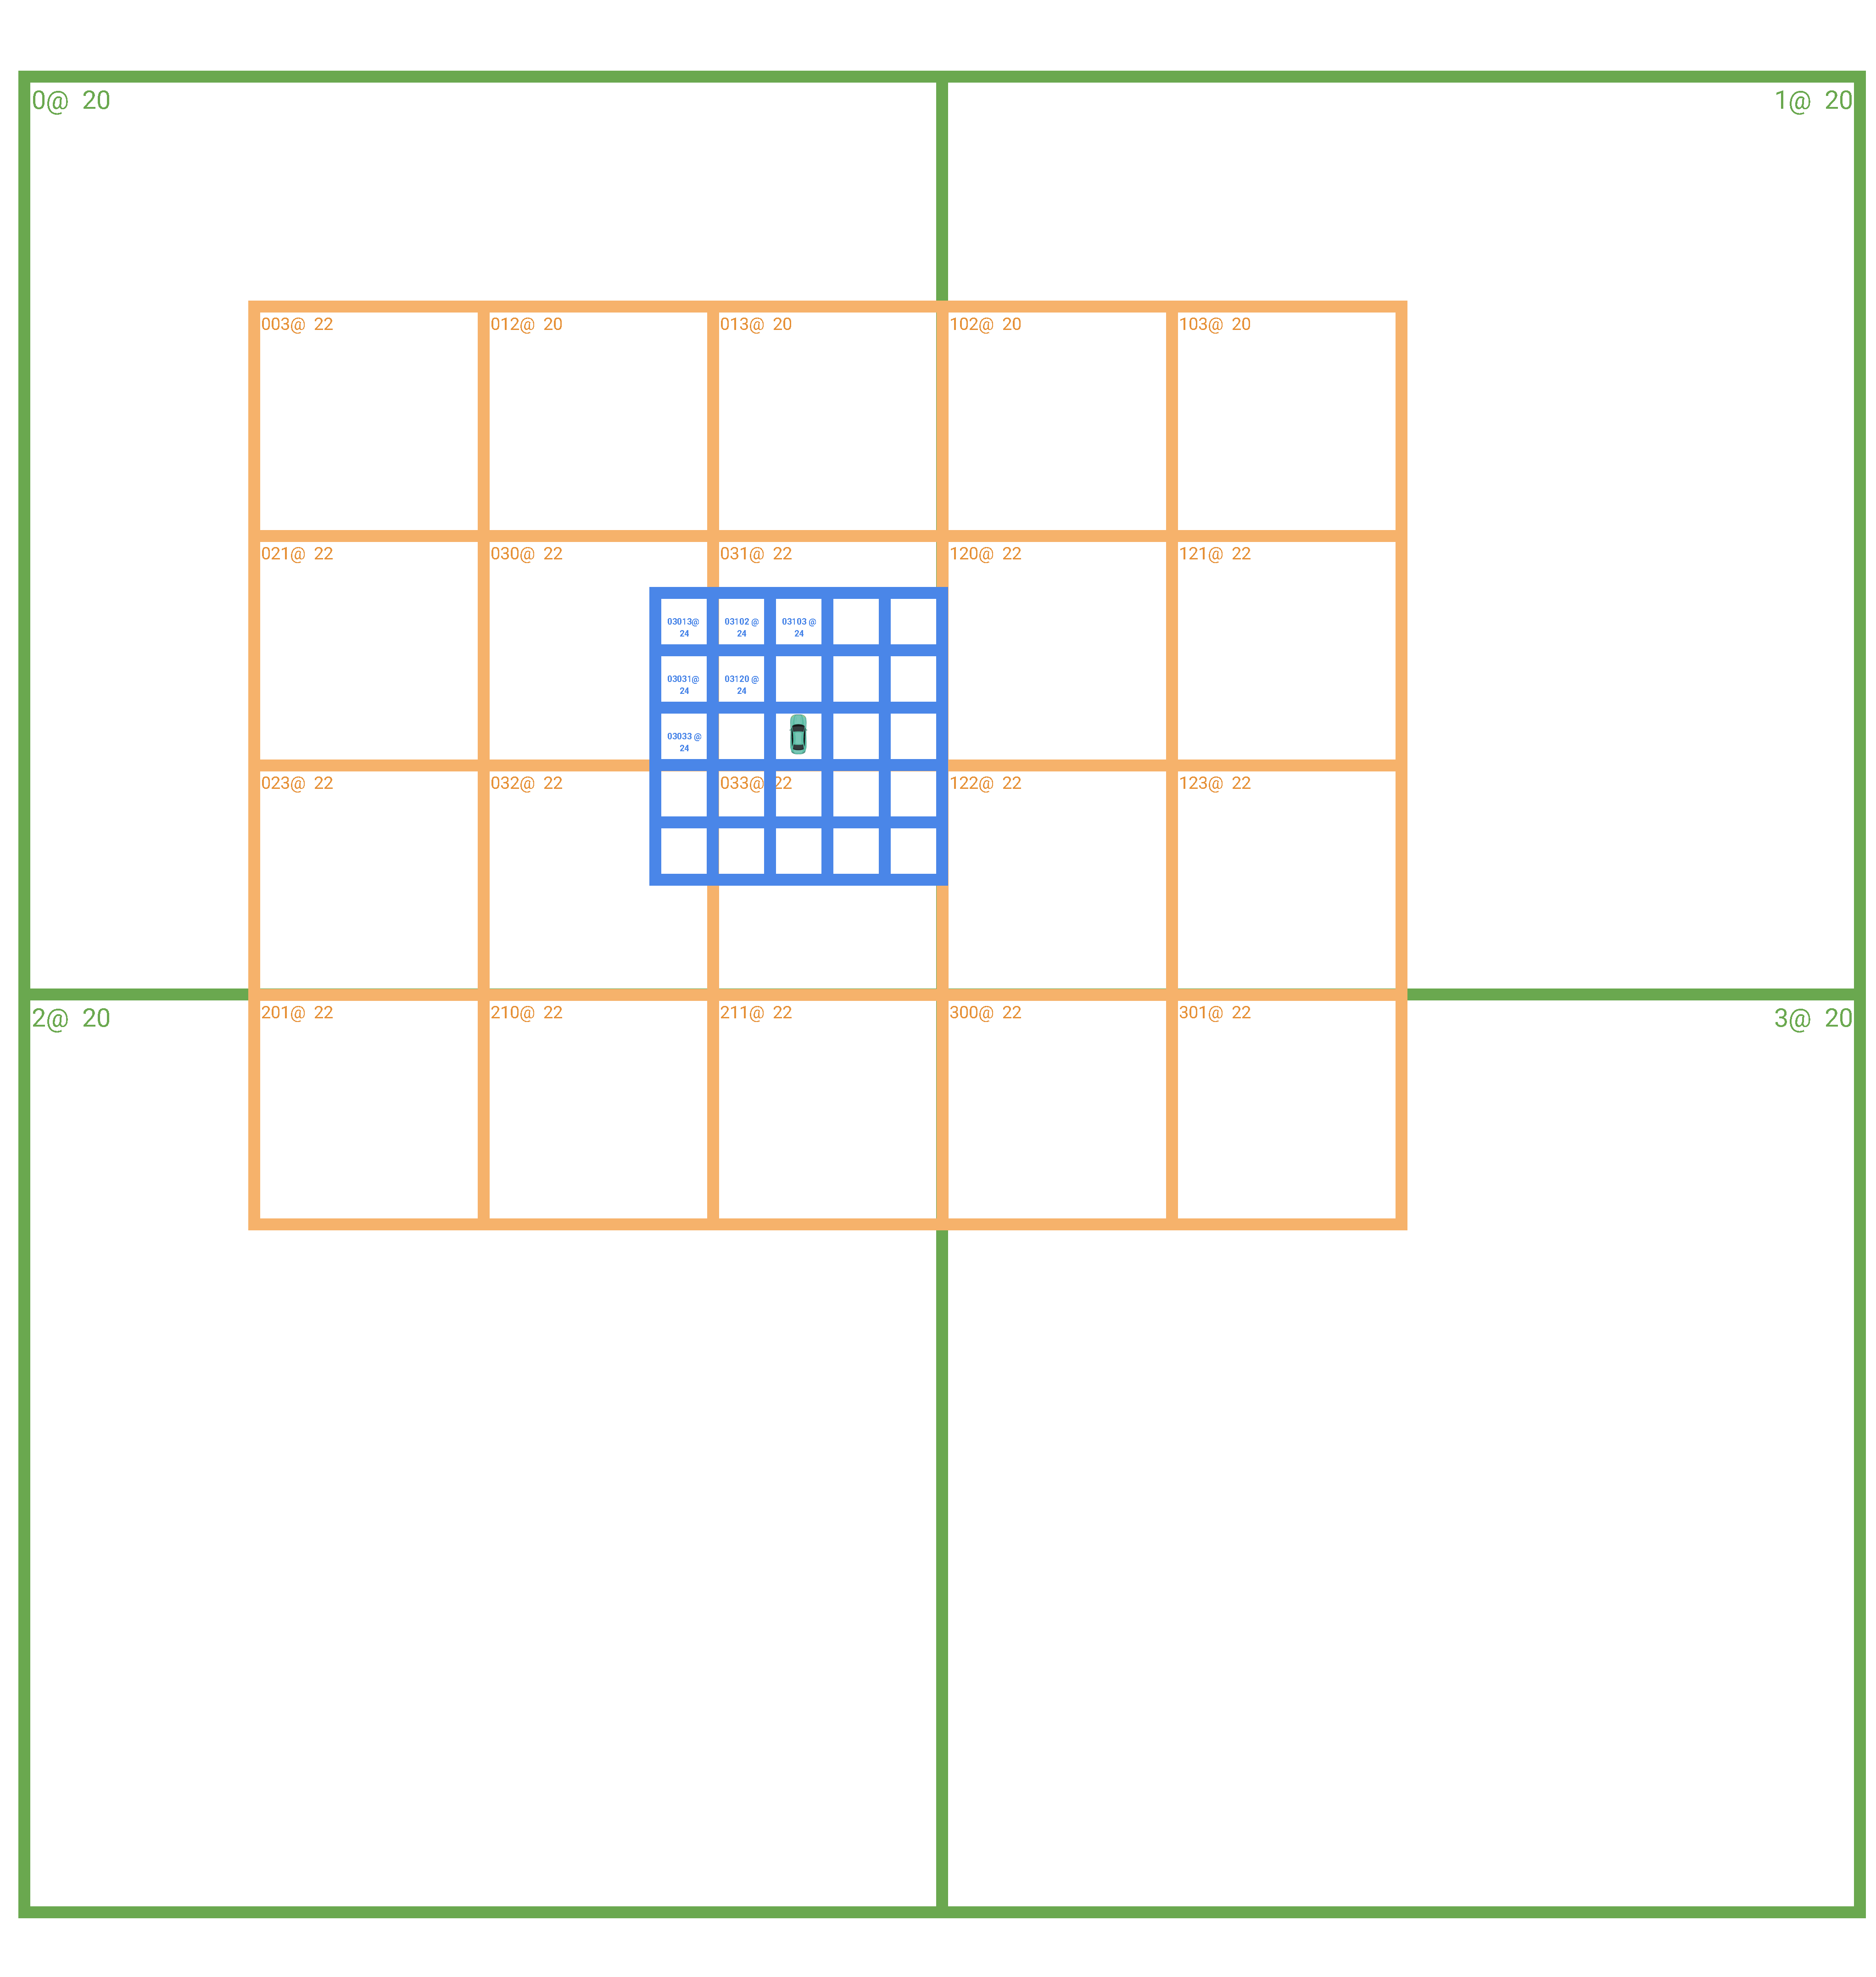
\includegraphics[width=0.9\linewidth]{98_images/geo_subscription_schema}
	\caption[Schematic Illustration of Geographical Sharding]{Schematic Illustration of Geographical Sharding \\ Blue cells (= type 1 tiles) are part of the vehicle's observed occupancy grid. \\ Orange cells (= type 2 tiles) are part of the vehicle's range of interest. \\ Green cells (=type 3 tiles) are subject to geo distribution.}
	\label{fig:geo_distribution_schema}
\end{figure}

\subsection{Messaging \& Further Considerations}
\label{subsec:concept_design:messaging_further_considerations}
Up to this point, a high-level system architecture was proposed and the concept of geographical sharding was introduced as a solution to horizontal scalability. Complementing previous design decisions, this section formulates the exact communication pattern between clients (vehicles, pedestrians, etc.) on the one hand and the fusion node (RSU) on the other from an application-layer perspective. In addition, further considerations regarding the messaging protocol are made.
\par
\bigskip

In essence, two different patterns for communication in a client-server architecture can be thought of. First, there is the \textit{request-response} (req/res) pattern, according to which a client explicitly "'asks"' the server for certain information and potentially receives an "'answer"' to its request. This type of communication is unidirectional and most used throughout today's web. The second pattern is \textit{publish-subscribe} (pub/sub). Compared to req/res, it inverts the control flow to some extent. Instead of having the client (repeatedly) asking for new data, the server keeps providing such "'automatically"' and just as it appears after the client had initially expressed its interest once. Depending on the concrete implementation, this type of communication can be uni- or bidirectional. Both patterns come with their respective advantages and downsides and are each suitable for certain use cases.

The system proposed in the context of Ko-HAF \cite{Hohm2019} utilizes both: req/res to send and receive static- and meta information and pub/sub to exchange time-critical data. For CP use cases, most information is time-critical. Assuming observations, i.e. instances of the occupancy grid-based meta model presented in \autoref{sec:concept_design:environment_modeling_state_representation}, are continuously produced and fused at a constant rate of \SI{10}{\hertz} for each observer, data needs to be distributed among the network as quickly as possible. Given these conditions, pub/sub shows to be the most suitable communication pattern, as it inherently supports these types of \textit{data streaming} use cases and avoids additional overhead from repeatedly establishing new connections. As a consequence, communication between OBU and RSU is chosen to follow a \textbf{publish-subscribe} pattern with \textbf{periodic push} in the proposed system. The choice for a concrete pub/sub technology is deferred to \autoref{ch:implementation}. However, since usually a separate \textbf{message broker} is involved in pub/sub systems, such is already considered an integral system component. \autoref{fig:architecture} schematically illustrates the overall architecture for the proposed cooperative perception system.

\begin{figure}
	\centering
	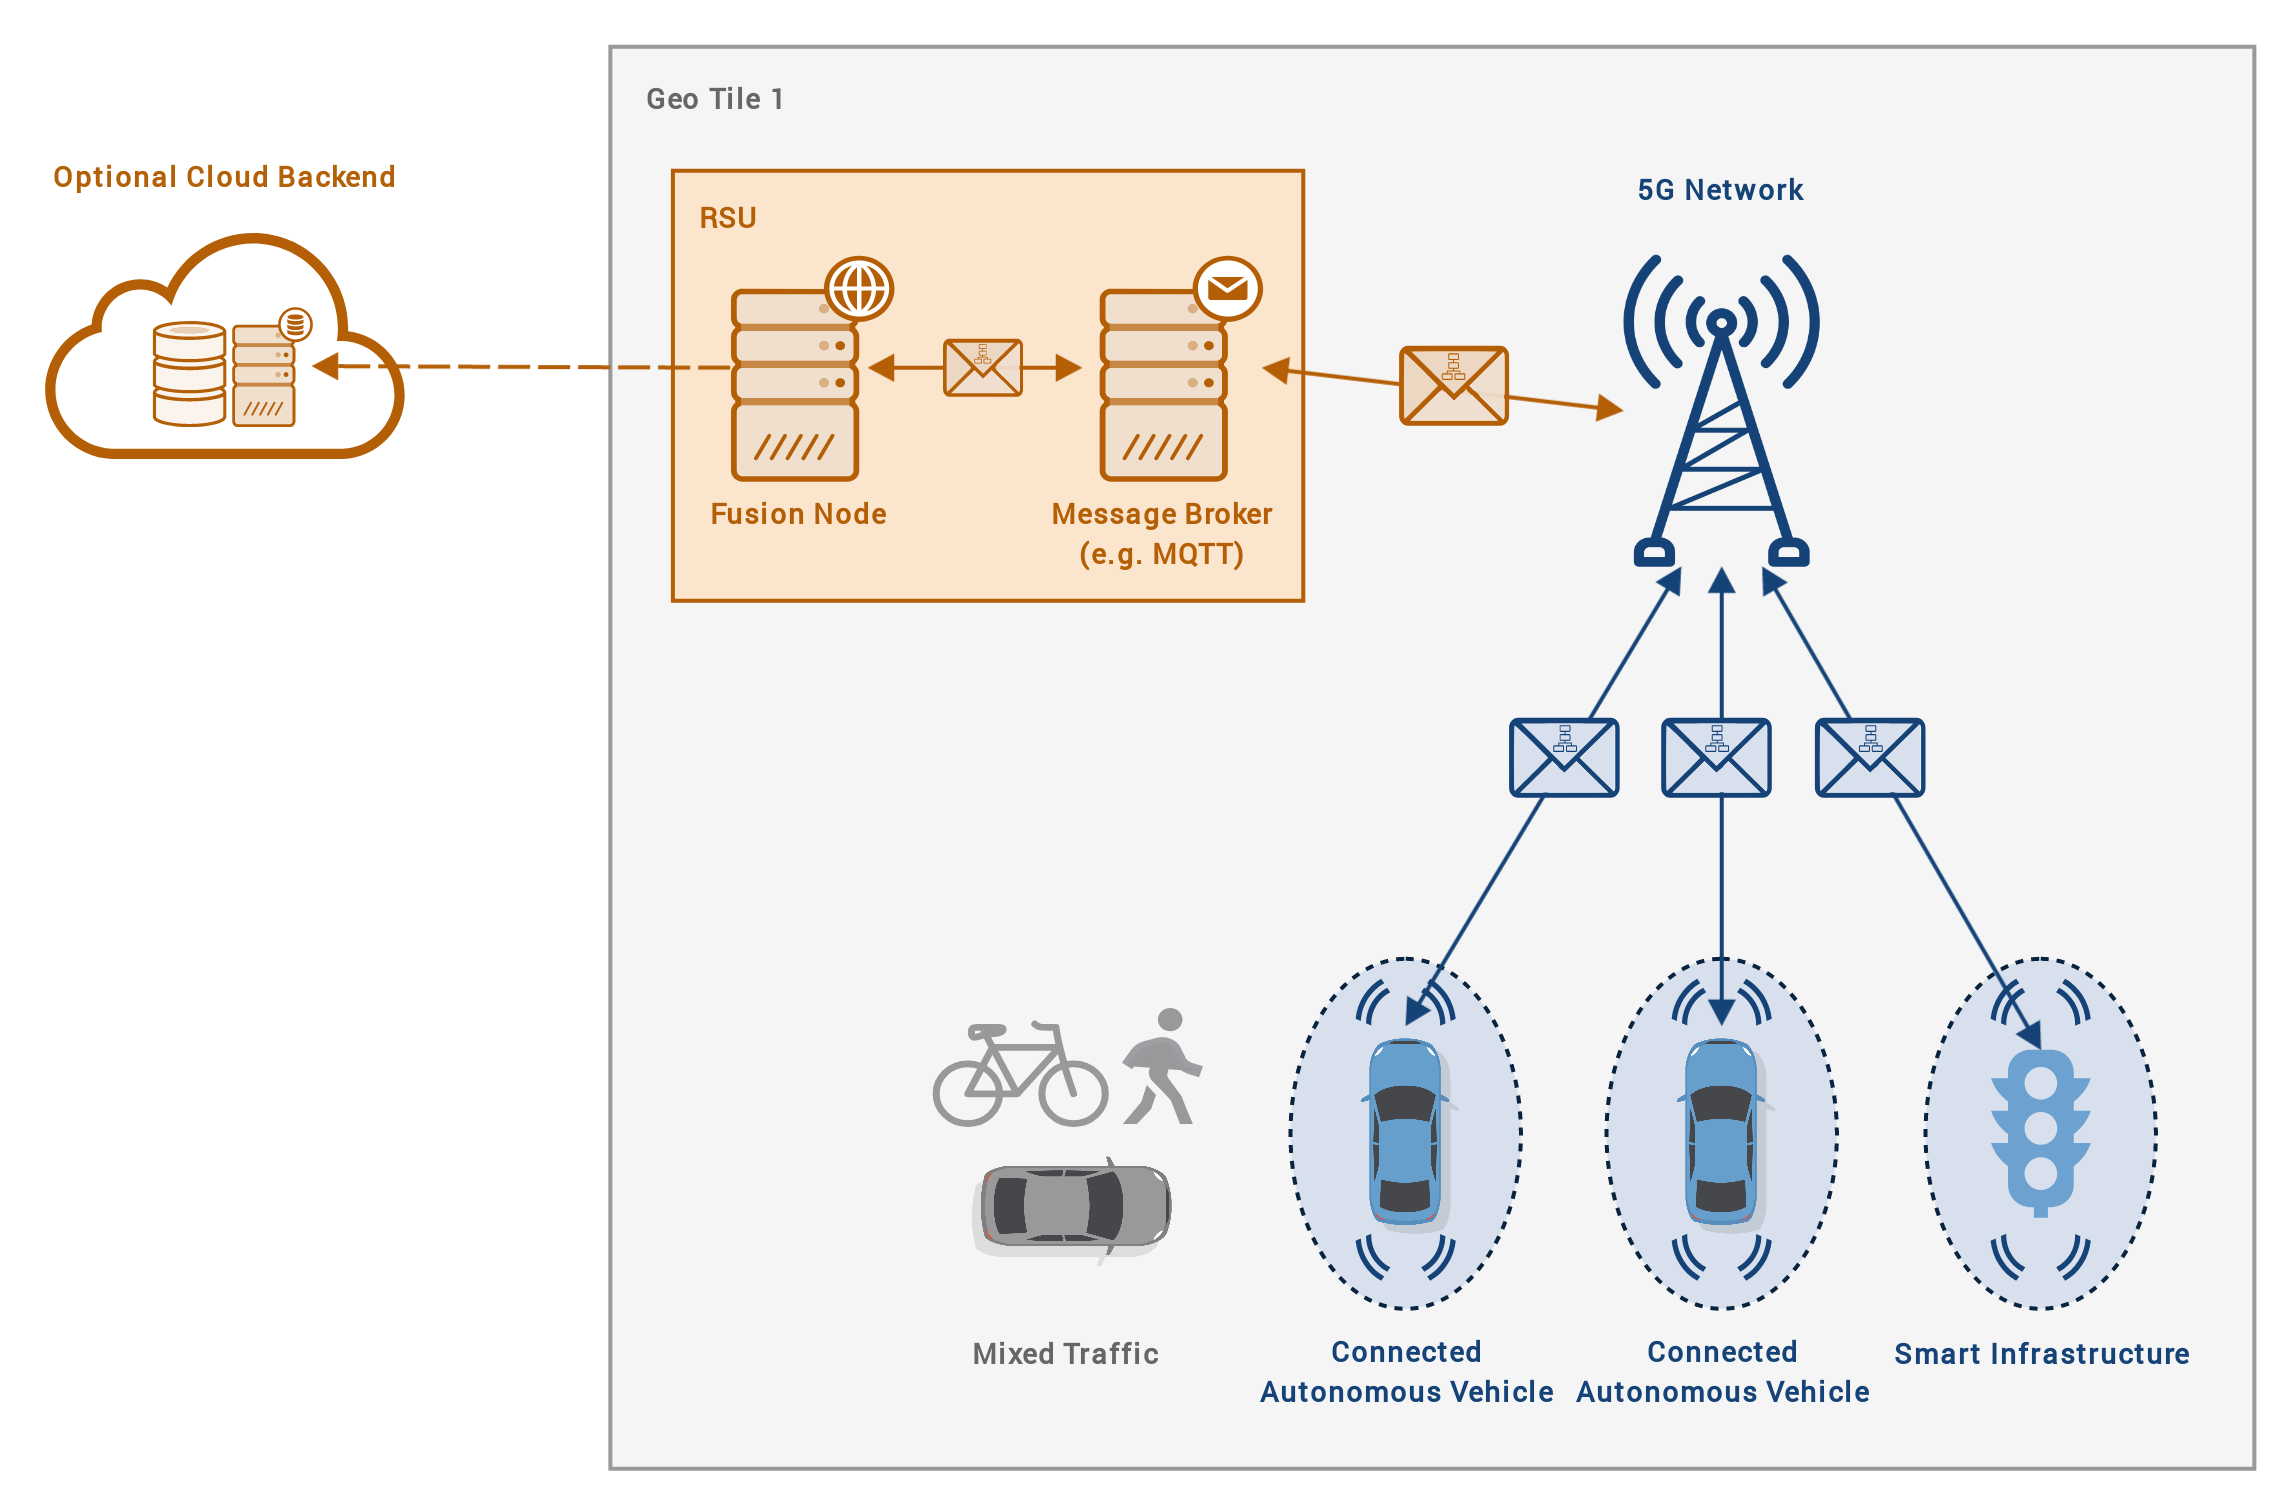
\includegraphics[width=1\linewidth]{98_images/architecture}
	\caption{Software Architecture Schema}
	\label{fig:architecture}
\end{figure}

\par
\bigskip

Another important aspect to be agreed upon is the representation format of data on the wire, or, in this case, on a wireless connection. Although \autoref{subsec:concept_design:probabilistic_entity_relationship_model_for_cooperative_perception} defined the environment model to be represented in form of a PER graph, no details have been provided on how to present that graph as a data structure. Since bandwidth is limited and latency must be kept low, a highly efficient (\textbf{NF-M3}, \textbf{NF-C3}, cf. \autoref{sec:problem_analysis:goals_requirements}) serialization format should be used. While the choice for a concrete technology is done in \autoref{ch:implementation}, a \textbf{binary serialization format} might be favored over more verbose, text-based formats like XML or JSON.


\subsection{Components Overview \& Summary}
\label{subsec:concept_design:components_overview}
After a high-level system architecture and respective communication patterns were elaborated, this section aims to provide a brief summary and an overview of all involved software components.

Unlike most previous takes on cooperative perception, our proposed system implements a client-server architecture with central fusion nodes to decrease network utilization and relieve the computational load on individual vehicles. It is holistic (\textbf{F-C1}) in such that covered aspects range from message representation over communication, scalability and fault-tolerance throughout to high-level sensor fusion (further discussed in \autoref{sec:concept_design:fusion}). To help scalability and reliability, the novel concept of geo sharding using QuadKeys is introduced and in accordance with requirement \textbf{NF-C4} (see \autoref{sec:problem_analysis:goals_requirements}) the system also allows for redundancy, i.e. multiple fusion nodes per type 3 tile, to avoid a single point-of-failure at the partition level. Communication between network participants happens on a publish-subscribe basis with the central fusion node implementing periodic push.

\autoref{fig:components_plain} shows a schematic overview of all components and relations among them. Each of these parts either already exists or is implemented in the course of \autoref{ch:implementation}.

\begin{figure}
	\centering
	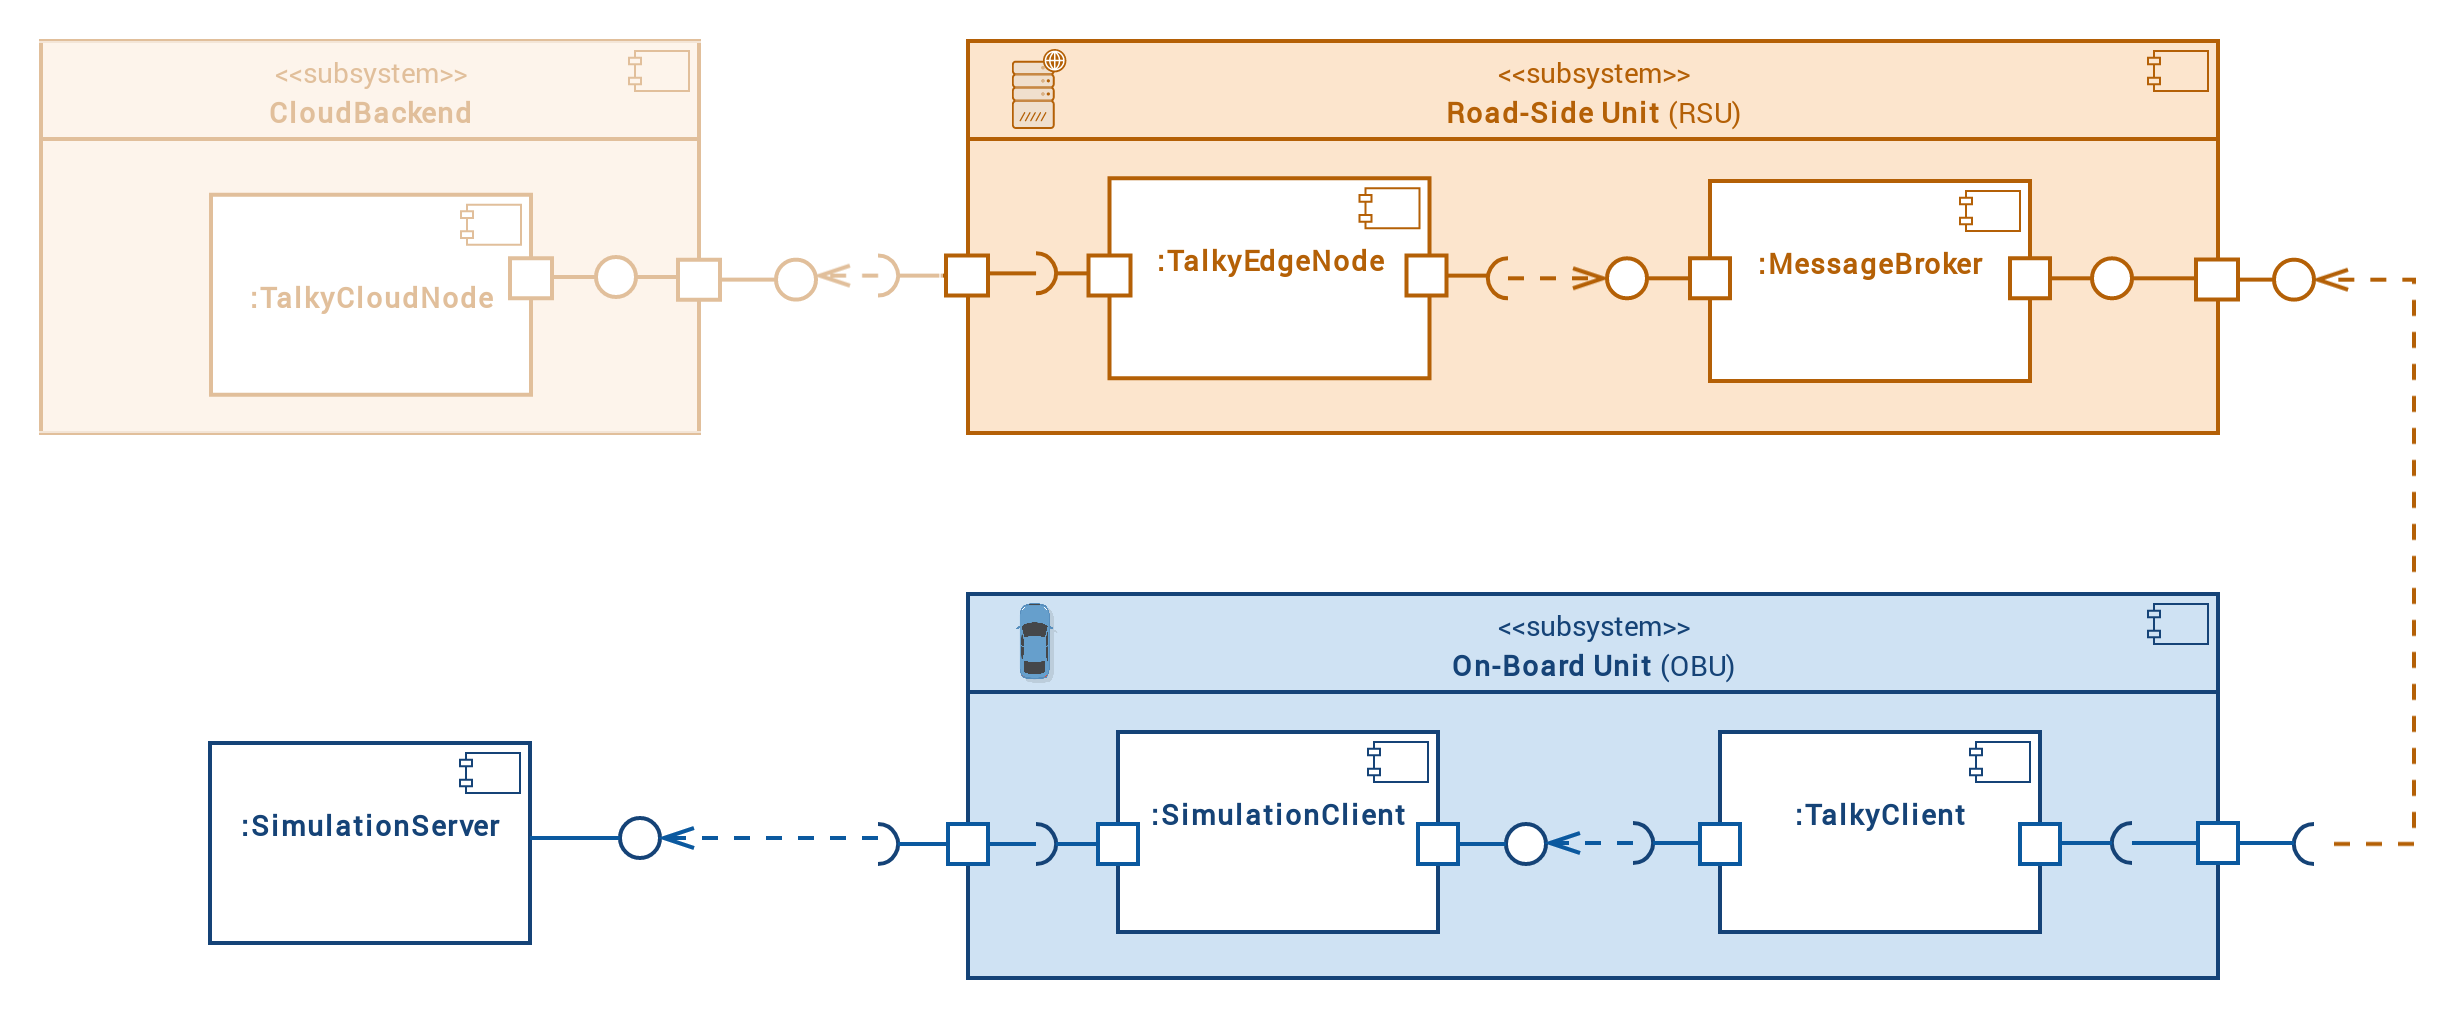
\includegraphics[width=1\linewidth]{98_images/components_plain}
	\caption{UML Component Diagram – System Architecture}
	\label{fig:components_plain}
\end{figure}

\begin{enumerate}[C1: ]
	\item \textbf{Simulation Server.} An integral part of this work is to integrate, test and evaluate the proposed solution with a simulator. Although the choice of which particular simulator to use is deferred to \autoref{ch:implementation}, we early agreed on employing a photo-realistic 3D simulator with a programmable interface. All existing solutions follow a client-server model, i.e. the simulation is executed on a central software component which is controlled by one or more clients through an API. The environment, weather, physics, traffic, sensory and more are simulated on this central server and usually it is also responsible for 3D rendering the scenes. Naturally, this component is only required for research purposes and would be omitted in a real-world deployment of the system.
	\item \textbf{Simulation Client.} This component lives within the \textbf{OBU subsystem}, i.e. is part of the collection of software that runs on-board of vehicles and other connected traffic participants. It belongs to the simulation infrastructure and is the counter-part of the previously mentioned simulation server, whose API it uses. This client acts as an intermediary between simulation environment and the actual CP system and is responsible for receiving and converting sensor- and meta data and sending control commands. It might be implemented as a separate software component or integrated into the on-board software suite as a module and is supposed to be implemented in a way that it abstracts from an actual underlying perception system from the Talky client's (see below) perspective. In other words, it simulates a real in-vehicle perception system and therefore is also responsible for low-level sensor fusion. Ideally, the interface, including inputs and outputs, is so generic that the fact of it being part of a simulation is transparent from the outside. Therefore, this component would be best realized following the \textit{Bridge} and \textit{Facade} design patterns (cf. \cite{EricFreemanElisabethFreemanBertBates2013}).
	\item \textbf{Talky Client.} As a core part of the actual CP system on the vehicle side, this component fulfills a variety of tasks. First, it is responsible for reading locally fused sensor data from the simulation client and building an occupancy grid from it. After being augmented with additional meta information about the observer and context, the grid is eventually embedded into an instance of the previously mentioned PER model, then serialized and sent to the currently responsible message broker. Simultaneously, the Talky client listens for new incoming messages from that broker, i.e. new cooperative perception messages originating from surrounding network participants, that were aggregated and fused at the server. These messages are then deserialized into a PER model instance again to reconstruct the shared scene representation and then, once again, fused with the latest local observation. Details on how the fusion process exactly looks like are presented in \autoref{sec:concept_design:fusion}. In a real-world use case, the resulting fused scene representation would eventually be input to the planning module within the AD pipeline (cf. \autoref{subsec:background:autonomous_driving_pipeline}) to help control the car more reliably. In this work, it is instead fed into the evaluation system to get insights about CP performance and more.
	\item \textbf{Message Broker.} The message broker is the first component to "'sit"' on the server-side of the system, i.e. "'on the other side"' of the intermediary 5G connection. That is, the \textbf{RSU subsystem} in the above schema. It should be physically close to both the cell tower and the edge node (see below) to achieve low latency. In pub/sub systems a message broker is commonly employed in the middle between multiple applications that communicate among each other via messaging. In essence, it is responsible for maintaining layer 4 network connections with all connected devices and receiving and properly forwarding messaging according to pre-defined policies. It abstracts low-level, messaging-related tasks, including authentication and authorization, from business applications. Several implementations already exist, however, which one to use usually depends on which pub/sub protocol is chosen. Examples include, but are not limited to different AMQP\footnote{http://www.amqp.org}- and MQTT\footnote{http://mqtt.org} brokers and are discussed in greater detail in \autoref{ch:implementation}.
	\item \textbf{Talky Edge Node.} Also referred to as fusion node or RSU, this component implements the concept of an edge server in the sense of edge computing \autoref{sec:background:edge_computing} and is the second core part of the presented CP system besides the above mentioned Talky client. It is the central server instance that is deployed once per type 3 tile as a \textit{geo shard}. Its core responsibilities include to aggregate every connected participant's state representation (via the message broker) and fuse all of them to a single, combined state representation, which is eventually published back to all connected Talky clients again following a \textit{periodic push} pattern. As all PER models produced within the corresponding type 3 tile at a rate of 5-20 \si{\hertz} are gathered here, this component has to be highly available, reliable, performant and equipped with a fast network connection.
	\item \textbf{Talky Cloud Node.} This component is part of a further level of abstraction on top of the previously presented edge node. Although it is optional and was not implemented as part of this thesis, it might be desirable in a real-world scenario. Similar to what the authors of \cite{Calvo2017} presented as third level of their multi-level cooperative perception scheme, the cloud node might be used for high-level tasks like navigation, traffic reporting or further analyses based on aggregated data from a multitude of different type 3 tiles. It could also be used as a central data lake for persistence. As the name suggests, this component would usually be deployed as one or few instances on the cloud and is another integral part of a typical edge computing architecture. 
\end{enumerate}

\section{Fusion}
\label{sec:concept_design:fusion}
In addition to a model specification (\autoref{sec:concept_design:environment_modeling_state_representation}), a communication- (\autoref{sec:concept_design:cellular_communication}) and overall system architecture (\autoref{sec:concept_design:system_architecture}), a concept on how to perform high-level sensor data fusion is required. Although this part is not particularly focused on in this work and might be elaborated in much greater detail and with more advanced methods in future research, basic considerations are still being discussed and an elementary concept is proposed. For the sake of clarity it is worth emphasizing that this section only concerns about the high-level fusion performed on client (C3) and edge node (C5), as opposed to low-level sensor fusion within the on-board perception module or, in this case, the simulation client (C1).

\subsection{Goals}
\label{subsec:concept_design:fusion_goals}
Essentially, the goals of fusion in a cooperative perception system are (1) to \textbf{supplement or impute missing data} and (2) to \textbf{increase the confidence} for existing data. The latter also includes to \textbf{resolve conflicts} and contradictory observations. (1) is essential for virtually perceiving a scene beyond the observer's own line of sight. (2) helps to increase accuracy and overcome sensor noise. \autoref{fig:fusion_goals_1} and \autoref{fig:fusion_goals_2} depict simplified examples, respectively, in which the occupancy state of cells are subject to fusion.
\par
\bigskip

\begin{figure}[h]
	\centering
	\begin{subfigure}[b]{1\textwidth}
		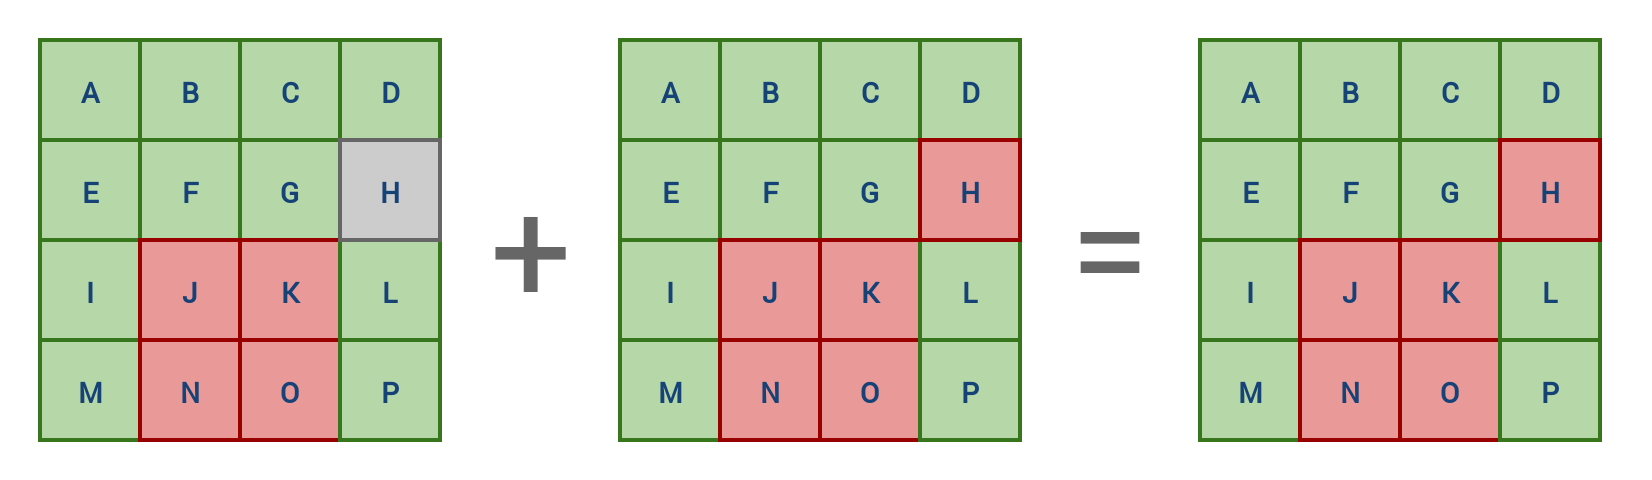
\includegraphics[width=0.9\linewidth]{98_images/fusion_goals_ex1}
		\caption{Schematic Example for Supplementation through Fusion}
		\label{fig:fusion_goals_1}
	\end{subfigure}
	
	\begin{subfigure}[b]{1\textwidth}
		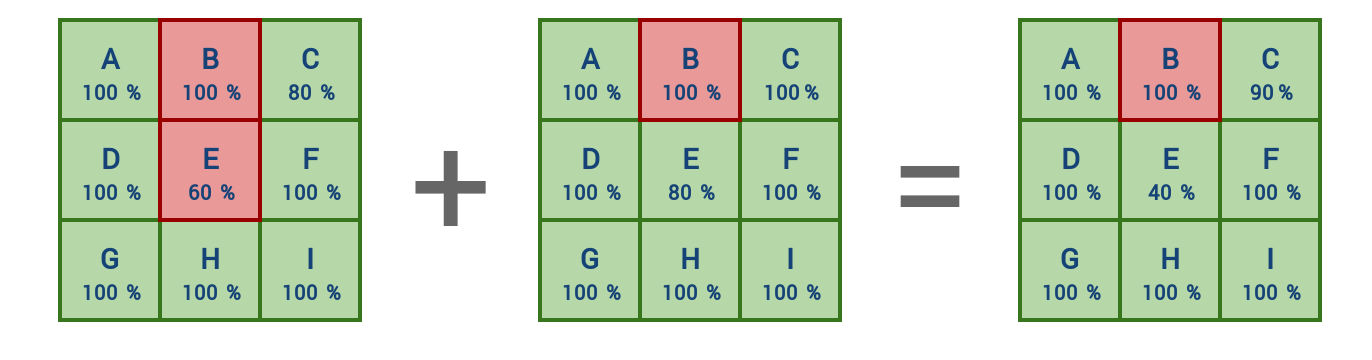
\includegraphics[width=0.89\linewidth]{98_images/fusion_goals_ex2}
		\caption{Schematic Example for Conflict Resolution through Fusion}
		\label{fig:fusion_goals_2}
	\end{subfigure}
\end{figure}

In \autoref{fig:fusion_goals_1}, vehicle X observes the occupancy grid on the left and vehicle Y the one on the right. Green cells are considered free, red cells are considered occupied and for gray cells no state could be determined, e.g. due to sensor noise or because they were out of sight. Vehicle X failed to estimate the state for cell H, while vehicle Y measured it to be occupied. Accordingly, the fused grid includes cell H with a state of being occupied.

While confidences were omitted for the sake of simplicity in the first example, \autoref{fig:fusion_goals_2} includes them as well. In this scenario, emphasis is to be placed on cells C and E. While vehicle X is only 80 \% confident about the state of cell C, vehicle Y is perfectly sure about it being free. Accordingly, the resulting state has an average confidence of 90 \%. Moreover, a conflict exists for cell E. Vehicle X is 60 \% confident, that it is occupied, while vehicle Y is 80 \% confident of it being free. When neglecting all other factors (like time), the average confidence for each cells state might be used during the fusion to get a result of cell E being free with a confidence of 40 \%. Please note that these examples are drastically simplified.

\subsection{Problem Statement}
\label{subsec:concept_design:fusion_problem_statement}
Complementing the previous section, which informally stated the goals of fusion in the context of CP and provided two illustrative examples, a bit more formal problem definition is presented in the following.

As already mentioned in \autoref{subsec:background:sensor_fusion}, Elmenreich et al. define the problem of sensor fusion as \textit{"'the combining of sensory data or data derived from sensory data such that the resulting information is in some sense better than would be possible when these sources were used individually"'} \cite{Elmenreich2002}.
\par
\bigskip

More formally, for every type 3 tile with $n$ participants (e.g. vehicles), let $M^{loc}_i(t), i \in [0..n]$ denote the model instance that was obtained at vehicle $i$ at time $t$ and assume the participant with $i = 0$ is the ego vehicle, whose perspective is taken in the following. As explained in \autoref{subsec:concept_design:probabilistic_entity_relationship_model_for_cooperative_perception}, the model $M$ essentially consist of a set of quadruples $r$, which correspond to probabilistic relations of a graph. That is:

\begin{gather*}
	M^{loc}_i(t) := \{r_{i,0}(t) \ .. \ r_{i,m}(t)\} \\ 
	\text{with\ } r_{i,j}(t) \in \{ \langle \mathcal{E} \times \mathcal{A} \cup \mathcal{R} \times \mathcal{E} \cup \mathcal{L} \times \Gamma \rangle \} \\
	\text{and} \  \Gamma := \{ \gamma \in [0, 1] \subset \mathbb{R}^+ \} \\
\end{gather*}

The goal of fusion is, given every participants local model $M^{loc}_i$, to get an augmented model $M^{aug}_i$ that involves all other participants' relevant observations as well.

\begin{gather*}
	\text{Given\ } M^{loc}_0(t-1) \text{\ and\ } \{M^{loc}_i(t - \Delta t^{min}_i)\ |\ i > 0, \Delta t^{min}_i > 1\} \\
	\text{we look for\ } M^{aug}_0(t) \\ 
	\text{\ s.t.\ } \bigl|  M^{aug}_0(t) \bigl| > \bigl| M^{loc}_0(t-1) \bigl| \\
	\text{\ and\ } \psi(M^{aug}_0(t), M^{*}_0(t)) > \psi(M^{loc}_0(t-1), M^{*}_0(t))
\end{gather*}

$\psi$ denotes the evaluation or scoring function that compares the latent true environment state $M^*$ to the observed one. $\Delta t^{min}_i$ denotes the minimum fusion- and transmission latency for participant $i$, i.e. the temporally closest timestamp greater than $t$. 

A more detailed description of how this augmented model is gained through fusion is given in \autoref{subsec:concept_design:fusion_architecture}.

\subsection{Scope}
\label{subsec:concept_design:scope}
Before introducing the high-level fusion concept, the scope of fusion needs to be set. In principle, \textbf{all attributes and relations} in the model (see \autoref{subsec:concept_design:the_final_model}) can be subject to fusion. To fuse attributes means to "'merge"' or aggregate multiple values for the same attribute, as demonstrated for the \textit{state} attribute in \autoref{fig:fusion_goals_2}. To fuse relations means to reason about their existence between two given entities. Naturally, this requires some kind of tracking and matching to uniquely identify entities across multiple observers, which is non-trivial problem and subject to current research.

Attributes and relations might be categorized as clusters, for each of which a separate fusion mechanism applies. For instance, when fusing cell occupancy states, a potential fusion technique might be to take a weighted average for the binary truthfulness of every possible state and determine the argmax subsequently. Similarly, when attempting to merge different values for an attribute that describes a spatial position, one might use the weighted average Euclidean distance during fusion. However, one might also come up with more advanced mechanisms. For the sake of simplicity, only the fusion of cell occupancy states is implemented in this work. However, the given framework can easily be extended to support more fusion subjects and mechanisms. The exact procedure of fusing cell states is presented in \autoref{subsec:concept_design:fusion_mechanism}.

\subsection{Open- \& Closed World Assumption}
\label{subsec:concept_design:fusion_open_closed_world_assumption}
As explained in the previous section, all attributes and relations of the model can be fused in principle. However, different fusion mechanisms and functions need to be implemented for different types of attributes (e.g. numerical vs. categorical or temporal vs. spatial). Moreover, a major distinction has to be made for what to assume as an attribute's domain. Depending on the type or category of attribute, either the  \textbf{Open World Assumption (OWA)} or the \textbf{Closed World Assumption (CWA)} is appropriate. Which one is used has fundamental influence on the fusion result.

Taking a CWA means that – generally speaking – a logical statement, that is not known to be true, is considered false. Contrary to that, the OWA "'allows"' to have incomplete knowledge and does not consider \textit{negation as failure} \cite{wiki:neaf}. 

With respect to high-level fusion for CP, OWA vs. CWA plays an essential role when deciding what kind of fusion mechanism to use for different attribute classes. More precisely, it influences the way how confidences for entity-attribute- or entity-entity relations are interpreted. 

Generally, one could distinguish between attributes, whose domain is known and such, whose domain is not known. For the former, one could apply either CWA or OWA, while for the latter, the OWA has to be taken as a basis. For instance, while the domain for a ternary occupancy state is completely known (\textit{free}, \textit{occupied} and \textit{unknown}), the number of possible "'attribute"' values (i.e. entities as objects in a quadruple) is infinite for an entity-entity relation between different road participants. During the fusion, it is unknown how many potential vehicles, pedestrians and other traffic participants are in a scene and could potentially occupy a certain cell or not.

\subsubsection{Example}
Assume the observations from two different observers for the same situation are present and we want to fuse their estimations of the occupancy state of a certain cell. According to our model definition, both observers report exactly one quadruple for this cell's state each. Observer A reports $r_{1,A} = \langle \textit{cell}_i, \textit{hasState}, \textit{free}, 0.9 \rangle$ and observer B reports $r_{1,B} = \langle \textit{cell}_i, \textit{hasState}, \textit{occupied}, 0.8 \rangle$. Taking the CWA, the reported confidences may be interpreted as probabilities and since all possible states are known, the trivial assumption could be made that the two remaining unknown state values equally share the remaining probability mass. As a consequence, the following quadruples could be inferred:

\begin{gather*}
	r_{2,A} = \langle \textit{cell}_i, \textit{hasState}, \textit{occupied}, 0.05 \rangle \\
	r_{3,A} = \langle \textit{cell}_i, \textit{hasState}, \textit{unknown}, 0.05 \rangle \\
	r_{2,B} = \langle \textit{cell}_i, \textit{hasState}, \textit{free}, 0.1 \rangle \\
	r_{3,B} = \langle \textit{cell}_i, \textit{hasState}, \textit{unknown}, 0.1 \rangle \\
\end{gather*}

Applying a simple arithmetic average over the confidences of all observations for each possible state yields:

\begin{gather*}
	r_{1,\text{fused}} = \langle \textit{cell}_i, \textit{hasState}, \textit{free}, \gamma_1 \rangle \\
	r_{2,\text{fused}} = \langle \textit{cell}_i, \textit{hasState}, \textit{occupied}, \gamma_2 \rangle \\
	r_{3,\text{fused}} = \langle \textit{cell}_i, \textit{hasState}, \textit{unknown}, \gamma_3 \rangle \\
	\text{with\ } \gamma_1 = 0.5, \gamma_2 = 0.425, \gamma_3 = 0.075 \\
\end{gather*}

Taking the OWA, confidences can not be interpreted as probabilities, as the potential number of values is infinite. Instead, the trivial fusion approach from above would yield these quadruples when assuming an open world:

$$\gamma_1 = 0.45, \gamma_2 = 0.4, \gamma_3 = 0$$

As mentioned earlier, only the fusion of occupancy states is implemented in this thesis, for which the open-world assumption is used consistently.

\subsection{Mechanism: Time-Decayed Weighted Average}
\label{subsec:concept_design:fusion_mechanism}
This section describes how multiple observations for a single discrete, categorical attribute are fused. For the sake of simplicity, continuous attributes are disregarded and the focus is placed particularly on the fusion of cells' occupancy states. This state attribute's domain is discrete and finite (ternary). For instance, the statement that a cells is \textit{free} is binary, i.e. either true or false and an additional notion of uncertainty is incorporated by passing along a confidence value. The confidence values represents either attribute- or structure uncertainty (cf. \autoref{subsec:concept_design:probabilistic_entity_relationship_model_for_cooperative_perception}).
Despite this confidence, a fusion function also needs to respect the observation's temporal delay, i.e. its "'age"'. In a cooperative perception system, the presence of a transmission lag is inevitable and mainly arises from network latency. Accordingly, an observation is always outdated already when being fused. This degree of "'outdatedness"' is referred to as \textit{Reliability of Perception} by \cite{liu2013motion}, whose authors suggest to exponentially decrease it with increasing transmission lag. While the description of a scene that is a few millisecond old might still be quite accurate, but as it gets older, potentially several seconds, the scene has most likely changed too much to still rely on that state representation. 

We define the fusion function $\phi$ as a mapping from a set of model instances $\mathcal{M}$ (cf. \autoref{subsec:concept_design:probabilistic_entity_relationship_model_for_cooperative_perception}) and a real-valued temporal delay $\Delta t = t_{now} - t_{obs}$ to a new model instance.

\begin{gather}
	\phi: \mathcal{M} \times \mathbb{R}^+ \mapsto \mathcal{M}
\end{gather}

Accordingly, a fused model instance at time $t$ is given as:

\begin{gather}
	M^{fused}(t) = \phi(\bigcup^n_{i = 0} \bigcup^t_{u = t - \delta t^{max}} M^{loc}_i(u), t-t_i)
\end{gather}

$n$ denotes the number of observers and $\delta t^{max}$ is a user-defined parameter that specifies the maximum age of observations to include during fusion. Consequently, the input to the fusion function are all present observations (= PER model instances) from all present observers within the last $t - \delta t^{max}$ time steps.

Evaluating $\phi$ involves to evaluate the respective "'sub-"'functions to fuse the values of all certain entity-attribute ($\langle e, a \rangle$) or entity-entity (($\langle e1, e2 \rangle$)) combinations. Let these sub-functions be named $\varphi_{e,a}$ or $\varphi_{e1,e2}$, respectively. Moreover, the following function is defined to determine a \textbf{temporal decay factor} for every observation to weigh it by its degree of "'outdatedness"', just a proposed above.

\begin{gather}
	\textit{decay}(t_i) = \exp^{-\lambda * \Delta t} = \exp^{-\lambda * (t_{now} - t_i)}
\end{gather}

In this thesis, the above function is used globally throughout the entire fusion procedure to incorporate transmission lag.
\par
\bigskip

For a $\langle e, a \rangle$-combination whose value domain is categorical and finite, the \textbf{weighted arithmetic mean} can be used to aggregate (i.e. fuse) multiple evidences or observations. This is the method of choice implemented in this work to fuse occupancy states. Further fusion mechanisms for other types of $\langle e, a \rangle$- or $\langle e1, e2 \rangle$ combinations are considered to be out of scope and are not explicitly defined. In search for fill the placeholders $b$ an $\gamma$ of a $\langle e, a, b, \gamma \rangle$-tuple, one could follow a two-step procedure to determine the aggregated confidence value and actual attribute value.

\begin{gather*}
	\textit{maxconf}_{e,a} = \underset{b \in \textit{dom}(\langle e, a \rangle)}{\max} \frac{\sum_{j = 0}^{m} \textit{val}_b(r_j) * \textit{decay}(t_j)}{\sum_{i = 0}^{m} \textit{decay}(t_j)} \\\textit{maxval}_{e,a} = \underset{b \in \textit{dom}(\langle e, a \rangle)}{\arg\max} \frac{\sum_{j = 0}^{n} \textit{val}_b(r_j) * \textit{decay}(t_j)}{\sum_{j = 0}^{n} \textit{decay}(t_j)} \\
\end{gather*}

In the above equation, $\textit{val}_b$ is defined as

$$
\textit{val}_b(r) = 
	\begin{cases}
	\gamma \in r & b \in r \\
	0 & else
	\end{cases}
$$

and $m$ is the number of observations to be included into the current fusion that hold a quadruple containing $e$ at subject- and $a$ at predicate position. Moreover, sticking to the previous notation, $r$ denotes a relation quadruple as part of a model instance $M$.

Accordingly, the fused quadruple for this specific $\langle e, a \rangle$-combination would be $r_{i,fused} = \langle e, a, \textit{maxval}_{e,a}, \textit{maxconf}_{e,a} \rangle$.

\subsection{Architecture: Doubly Updated Merging}
\label{subsec:concept_design:fusion_architecture}

While the previous section gave an in-depth description of how a single entity-attribute combination might be fused, this section returns back to a higher-level perspective and examines the fusion process in its whole again.

The concept of \textit{doubly updated merging} is introduced as a technique to address the fact that an observation is delayed twice on its way through the CP system. First, as a local observation $M^{loc}_i(t)$, it experiences a transmission lag $\Delta t_1$ while being transferred from the on-board Talky client via the message broker to the fusion- / or edge node. After it was fused at the server and became part of $M^{glob}(t+\Delta t_1+\epsilon_1)$ it is transmitted all the way back to the client, which causes another delay $\Delta t_2$. While the server considered $\Delta t_1$ as a decay factor during fusion, the client needs to incorporate $\Delta t_2$ as well. Therefore, the client performs another round of fusion, in which $M^{glob}(t+\Delta t_1+\epsilon_1)$ and its latest local $M^{loc}_i(t+\Delta t_1+\epsilon_1+\Delta t_2+\epsilon_2)$ are merged into the final $M^{aug}_i$. This process is depicted as a sequential schema in \autoref{fig:sequence}.

\begin{figure}[H]
	\centering
	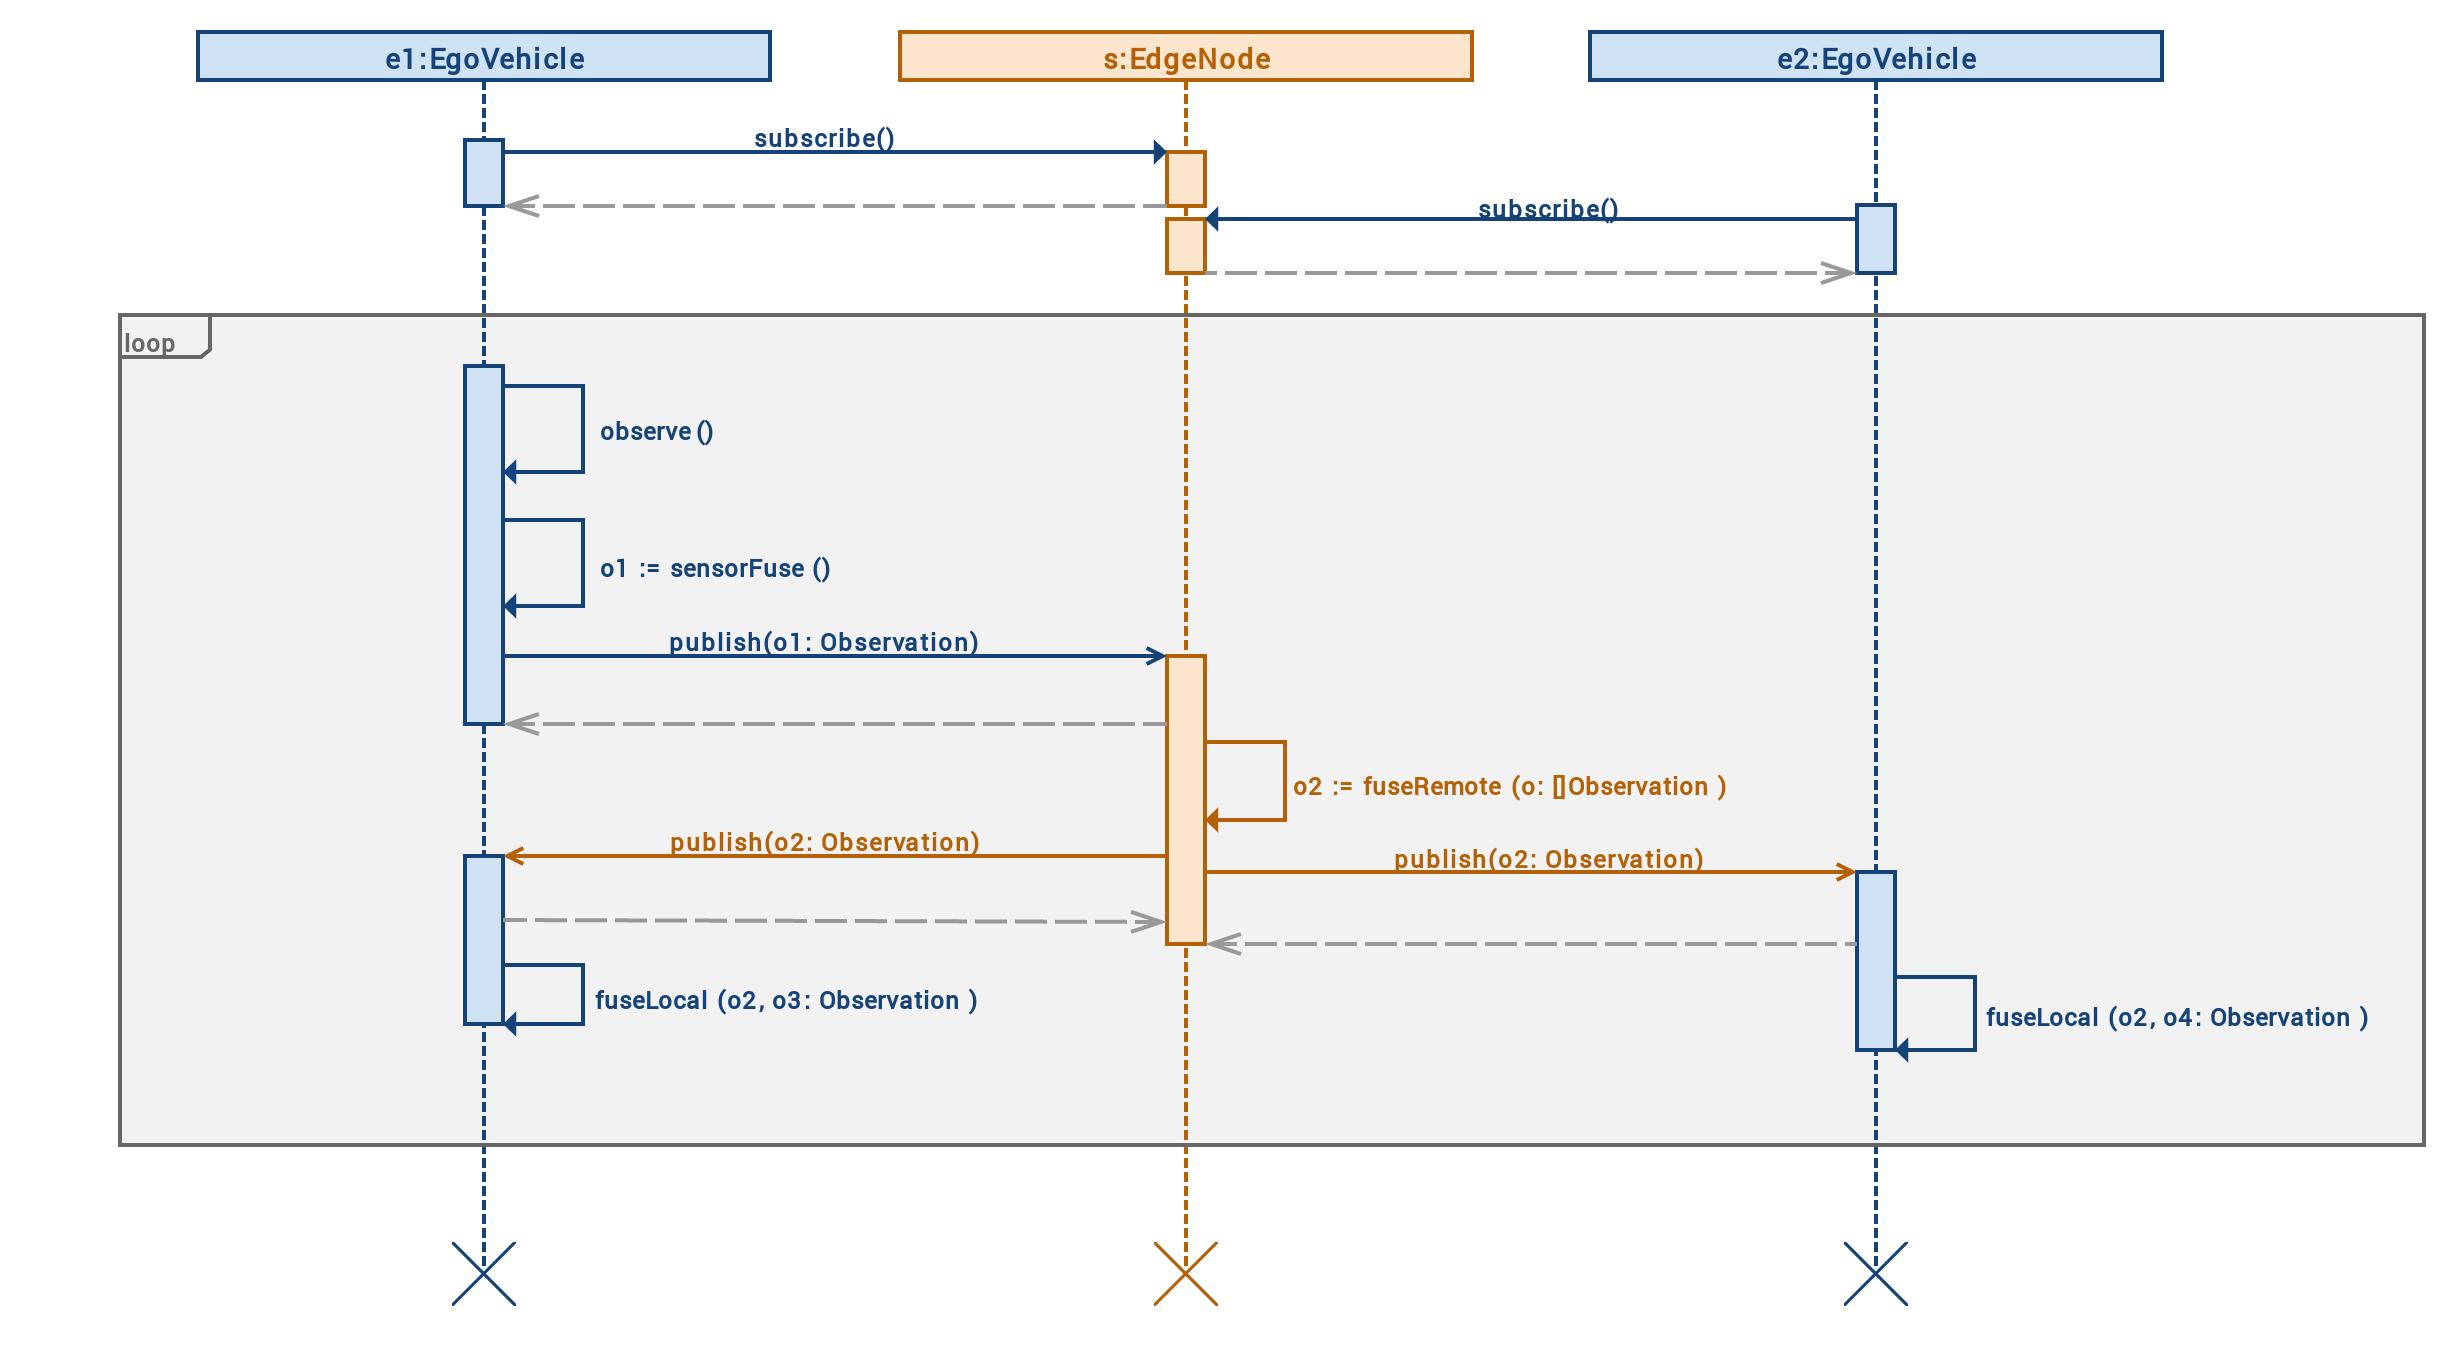
\includegraphics[width=1\linewidth]{98_images/sequence}
	\caption{UML Sequence Diagram – High-Level Fusion}
	\label{fig:sequence}
\end{figure}

Given the definition of relation quadruples $r$ in \autoref{eq:quadruples}, the three different state representations (or model instances) produced in the course of one iteration of \textit{doubly updated merging} can be formally stated as follows.

\begin{align}
	\textbf{Local:\ } &\  M^{loc}_i(t_0) = \{ r_{i,0}(t_0)\ ...\ r_{i,j}(t_0)\} \\
	\textbf{Globally Fused:\ } &\  M^{glob}(t_1) = \phi(\bigcup^n_{i = 0} \bigcup^{t_1}_{t = t_1 - \delta t^{max}} M^{loc}_i(t), t-t_i) \\
	\textbf{Locally Double-Fused:\ } &\  M^{aug}_i(t_2) = \phi(\{ M^{loc}_i(t_2), M^{glob}(t_1) \}, t_2 - t_1)
\end{align}
\begin{gather*}
	\text{with\ } \delta t^{max} > 0, t_2 > t_1 > t_0
\end{gather*}

\subsection{Summary}
\label{subsec:concept_design:fusion_summary}
Previous sections presented a very basic concept of how to perform high-level sensor fusion in a cooperative perception system, which is later implemented and evaluated in \autoref{ch:implementation} and \autoref{ch:evaluation}. 

However, since fusion is not the core aspect of this thesis, the previously presented techniques are only rudimentary and could be advanced dramatically. Current limitations include the above fusion approach's assumption that every time lag is precisely known, i.e. all involved devices' clocks are perfectly synchronized and additional delays (e.g. from sensor to controller) are disregarded. Elaborate methods to account for unknown time already exist in literature \cite{Julier} and could be applied as part of future work. Moreover, tracking and matching of entities across multiple frames and multiple observers is not considered at all. Finally, while the taken approach to decrease the influence of temporally "'old"' observations is the simple, better performance might be achieved through imputation of missing data or extrapolation of past measurements to current time \cite{Chen2019}. 